\clearpage
\section{DOCX Templates}
\label{sec:builder-feature-docx-templates}

A DOCX template is an ordinary Word file where you write the fixed text and put tags in double braces where variable data goes, such as the employee's name or the request number. When a user presses the action button on a record, KayanOS fills the tags from the record's data and downloads the document as Word or PDF. That way contracts and letters are produced with consistent wording and no manual copying. This page shows the template list and how to create a template; writing tags and working inside a template each have a page of their own.

\textbf{Path and who uses it:} “Builder” → “Core” → “DOCX Templates”. Managed by those with Builder administration; users run them from a button on the record.

\begin{rcnote}[Example: Horizon]
The system administrator writes the visit confirmation letter in Word, adds one tag for the request number and another for the visit date, uploads it as a template and links it to a button in “Visit requests”. They upload the letter from ① and test it after opening it from ③.
\end{rcnote}

\begin{figure}[H]
\centering
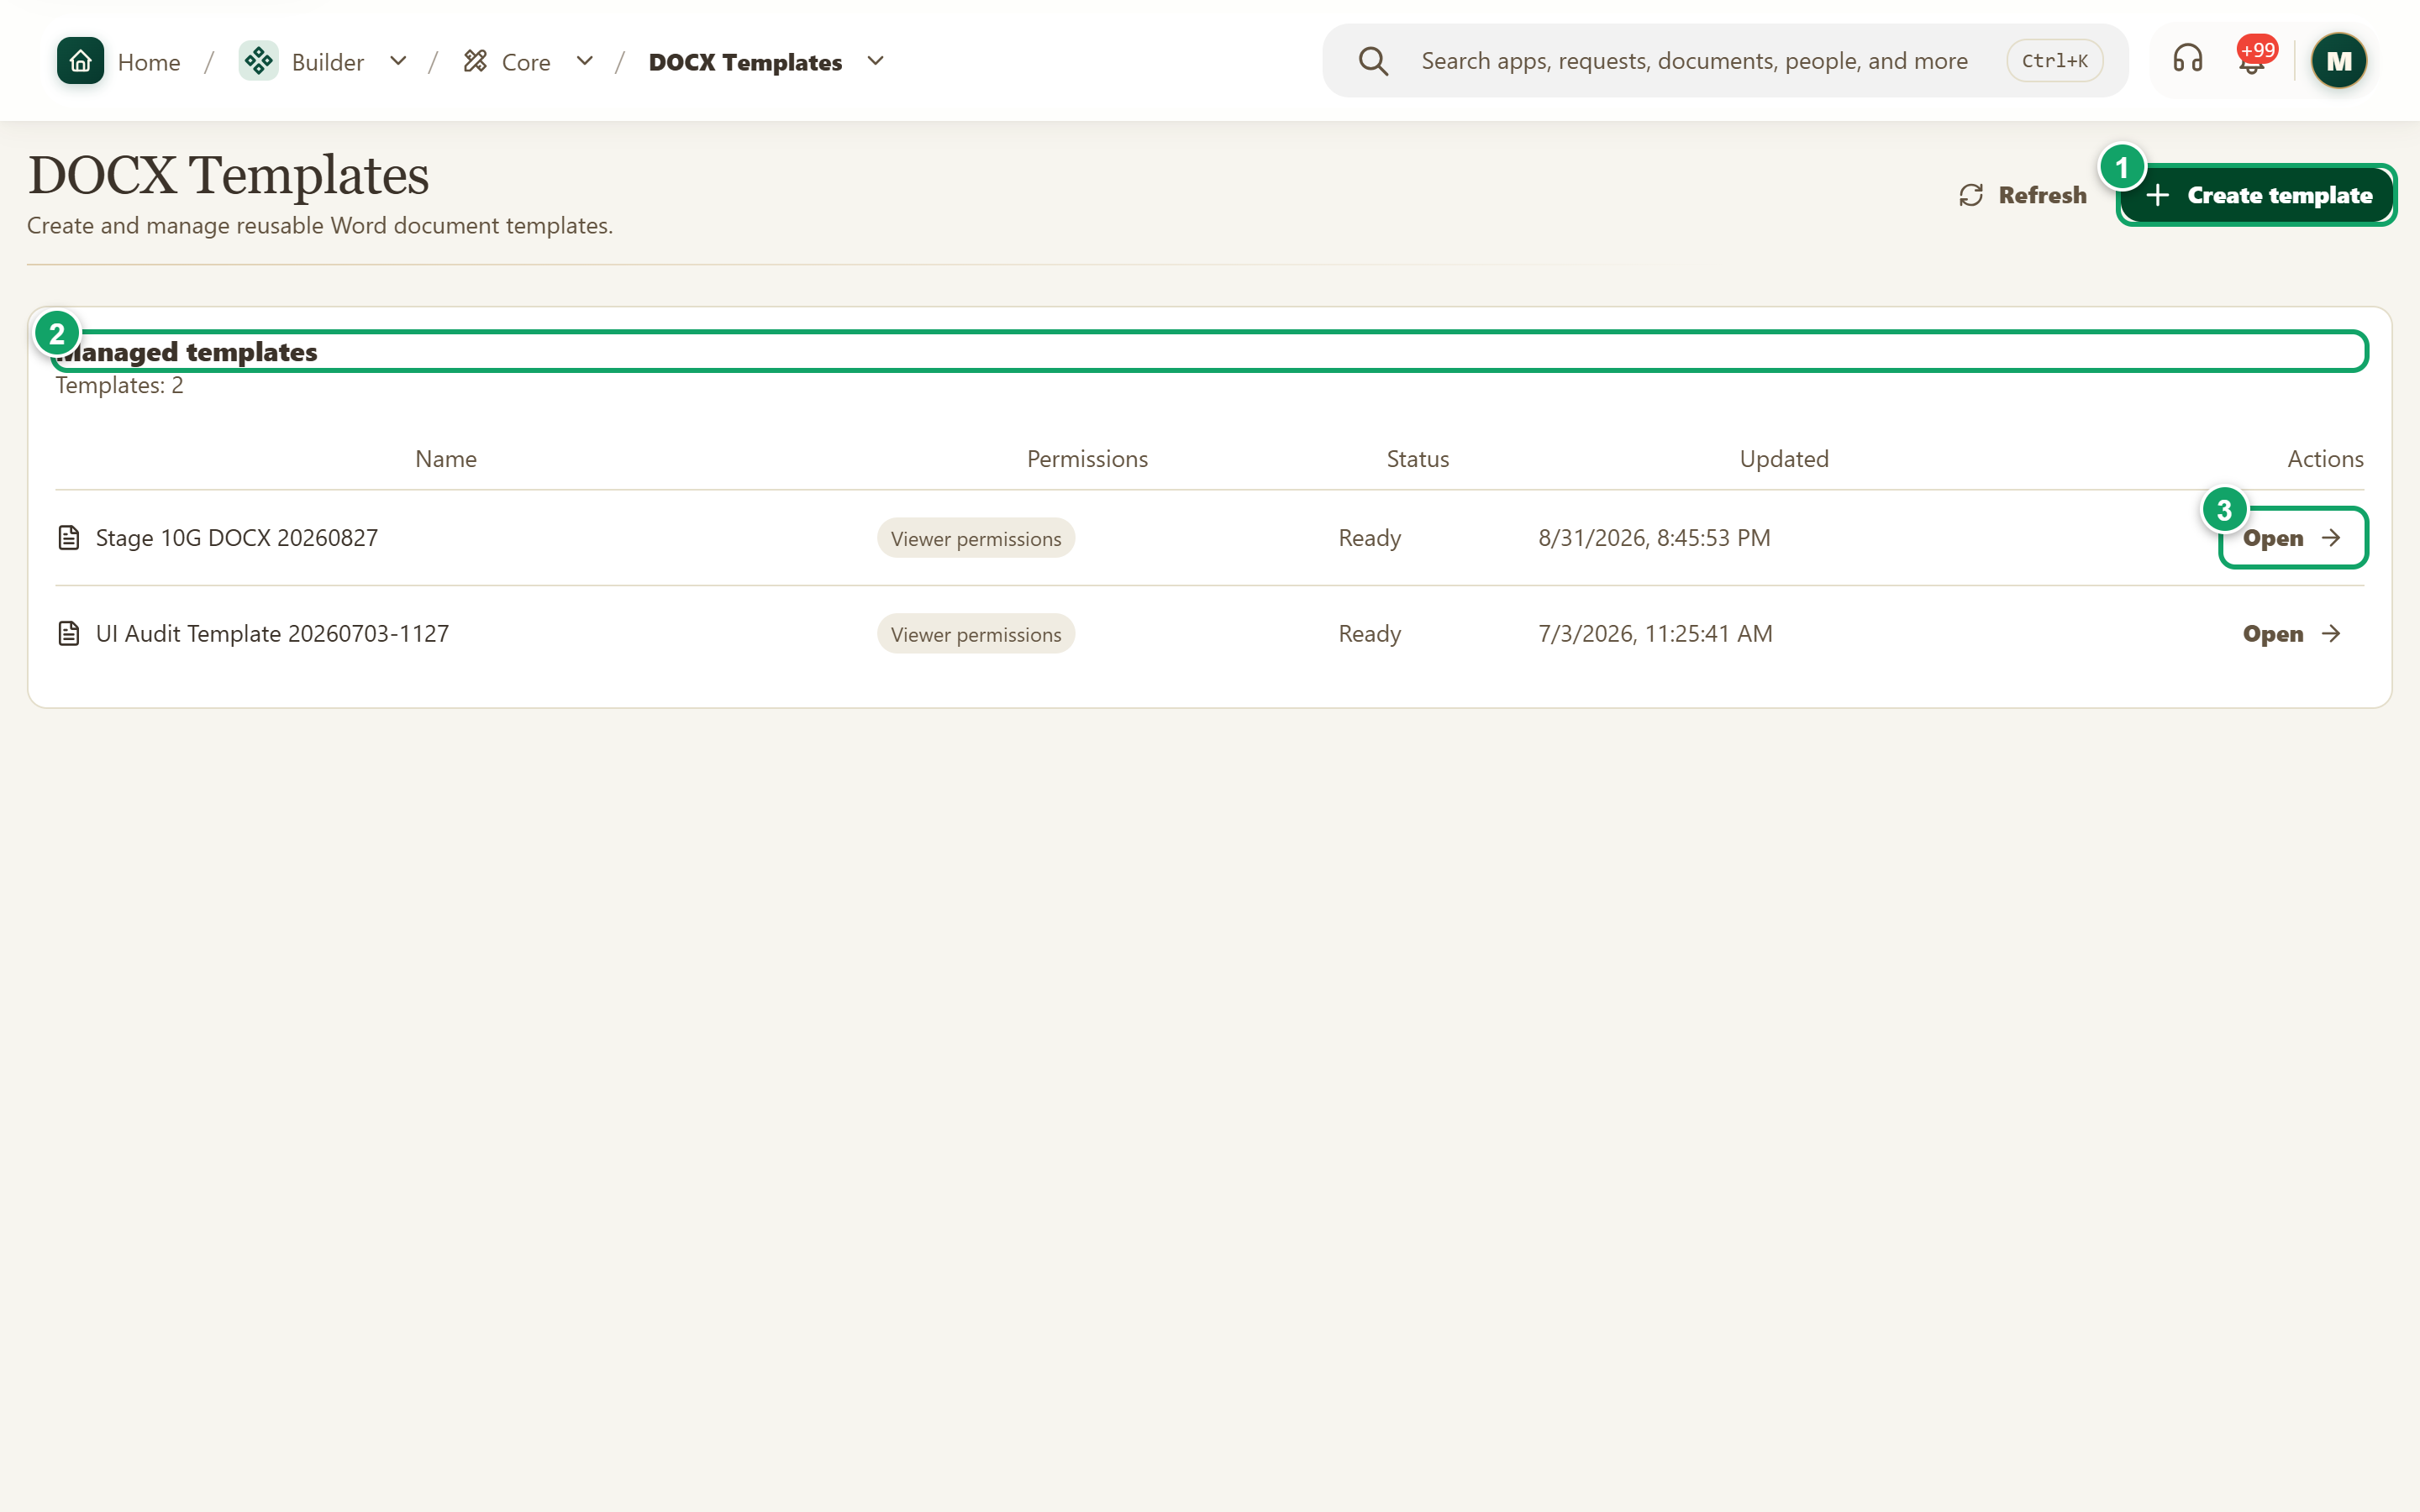
\includegraphics[width=0.95\linewidth,height=0.72\textheight,keepaspectratio]{figures/screens/ch06-docx-en.png}
\caption{The “DOCX Templates” page}
\label{fig:builder-docx-templates-screen}
\shotnote{The page lists managed templates with their permissions and status, here test templates. ① “Create template”: uploads a new Word file. ② “Managed templates”. ③ “Open”.}
\end{figure}


\begin{table}[H]
\centering
\caption{What do you find here?}
\label{tab:builder-docx-data}
\begin{tabularx}{\linewidth}{R{3.6cm} Y}
\rcHeaderRow
\thh{Part} & \thh{Content and action}\\
Managed templates & The list of templates with “Permissions” and “Status”: “Ready” when a current version exists, or “Needs a Word document”.\\
Create template & Upload a “Word document” in \en{.docx} format only, and write the “Template name” and “Description (optional)”.\\
Downloaded file name & Found under “Advanced defaults” and written as an expression that builds the name from record data, such as the request number. If it is blank or cannot be evaluated, the uploaded file name is used.\\
Document permissions & “Viewer permissions”, the recommended choice, show only what the downloader can see. “Administrator permissions” may put data in the document they cannot view.\\
Create with AI helper & A button shown when “AI in builders” is on; it starts the template with a helper that proposes a draft you review before saving.\\
\end{tabularx}
\end{table}

\begin{figure}[H]
\centering
\begin{tikzpicture}[node distance=0.5cm]
\node[stepBox] (a) {Word file with tags};
\node[stepBox,below=of a] (b) {Create and test the template};
\node[stepBox,below=of b] (c) {“DOCX template” action on the record};
\node[stepBox,below=of c] (d) {The user presses the button};
\draw[flowsTo] (a) -- (b);
\draw[flowsTo] (b) -- (c);
\draw[flowsTo] (c) -- (d);
\end{tikzpicture}
\rclegend
\caption{From a Word file to a document for every record}
\label{fig:builder-docx-flow}
\shotnote{The diagram shows that a template is not linked to a record type by itself; it reaches users through a “DOCX template” action you add in “Actions \& automations”. That is why testing on a real record comes before linking, because validation at upload does not catch every mistake in where tags are placed.}
\end{figure}

\subsection{Steps and check}
\begin{enumerate}
\item Write the document in Word, place tags using the real field keys, and put condition and loop tags in their own paragraph.
\item Open “DOCX Templates” and press “Create template”, upload the file, write the name and press “Create template”.
\item Open “Test \& download”, choose a record, then “Render and download” and review the document.
\item In the record type, add an action of kind “DOCX template” and choose the template in “Select template”, then publish.
\end{enumerate}

\textbf{Check and recovery:} the template's status should be “Ready”, and the action button should download a document filled with the record's data. If “This document needs attention” appears at upload, fix the listed tags and upload again. If a value is blank, check that you used the field's key, not its label.

\clearpage
\section{DOCX tags and loops}
\label{sec:builder-feature-docx-tags}

A tag is text in double braces that you write in the Word file where a value from the record should appear. KayanOS reads the tags when it creates the document and replaces them with data, in the body and also in page headers, footers, footnotes and comments. There are three kinds: a value tag placed inside a line next to other text, control tags for conditions and loops that take up a whole paragraph or a whole table row, and extra tags that insert an image, a link, a QR code or a page break.

\textbf{Path and who uses it:} tags are written in Word before uploading the file from “Builder” → “Core” → “DOCX Templates”. They are written by template managers, using field keys as they appear in the record type.

\begin{rcnote}[Example: Horizon]
In the visit confirmation letter, the system administrator writes the line “Visit date:” followed by the tag \en{\{\{ \$record.visit\_date \}\}}. Around that line they place a condition in its own paragraphs, so if no date is set yet the sentence “The date will be sent after review” appears instead.
\end{rcnote}

\begin{table}[H]
\centering
\caption{Tags and where they go in Word}
\label{tab:builder-docx-tags}
\begin{tabularx}{\linewidth}{R{3.6cm} Y}
\rcHeaderRow
\thh{Tag} & \thh{What it does and where it goes}\\
\en{\{\{ \$record.field\_key \}\}} & Inserts a field value by its key, not its label, and may share a paragraph with other text. An empty value prints as empty text.\\
\en{\{\{\#if ...\}\}}, \en{\{\{else\}\}} and \en{\{\{/if\}\}} & Show the paragraphs between them when the condition holds, otherwise what follows \en{else}. Each one sits alone in its paragraph or row.\\
\en{\{\{\#each list as item\}\}} and \en{\{\{/each\}\}} & Repeat the paragraphs or table rows between them for each item. Inside, \en{\$index} starts at zero, and \en{\$first} and \en{\$last} are available.\\
\en{\{\{@image ... width=120\}\}} & Inserts a PNG, JPEG or WebP image up to 10 MB; add \en{optional=true} when it may be absent.\\
\en{\{\{@link url label\}\}} & Inserts a link starting with \en{http}, \en{https} or \en{mailto} only.\\
\en{\{\{@qr ... width=120\}\}} & Creates a QR code from a non-empty value, such as the request number.\\
\en{\{\{@pageBreak\}\}} & Starts a new page.\\
\en{\{\{> ...\}\}} & Inserts the body of another template, such as a standard clause, alone in its paragraph. Up to five nested include levels are allowed.\\
\end{tabularx}
\end{table}

\begin{table}[H]
\centering
\caption{The data a template reads}
\label{tab:builder-docx-tags-context}
\begin{tabularx}{\linewidth}{R{3.6cm} Y}
\rcHeaderRow
\thh{Root} & \thh{What it holds}\\
\en{\$record} & The selected record's fields and general data, by key.\\
\en{\$inverseRelations} & The records that point to this record, as configured in the action.\\
\en{\$organization} and \en{\$member} & The current organization and the member creating the document.\\
\en{\$now} & The time the document is created; you format it yourself.\\
\en{getRecords} & A function that fetches records of another type, up to 500 records per call, under the downloader's permissions unless the template is set to “Administrator permissions”.\\
\end{tabularx}
\end{table}

\begin{rcwarn}[Upload validation does not guarantee tag placement]
Validation catches empty or unclosed tags and unsupported commands such as \en{@html}, \en{@chart} and raw XML insertion. But it does not guarantee that a condition or loop tag sits alone in its paragraph, so an upload can succeed and then text disappears or the tag prints. Test every condition and loop on a real record after each change.
\end{rcwarn}

\begin{figure}[H]
\centering
\begin{tikzpicture}[node distance=0.5cm]
\node[stepBox] (a) {Value tags inside lines};
\node[stepBox,below=of a] (b) {Condition and loop tags\\in their own paragraphs};
\node[stepBox,below=of b] (c) {Upload and validation};
\node[stepBox,below=of c] (d) {Test on a real record};
\draw[flowsTo] (a) -- (b);
\draw[flowsTo] (b) -- (c);
\draw[flowsTo] (c) -- (d);
\end{tikzpicture}
\rclegend
\caption{The order for writing and testing tags}
\label{fig:builder-docx-tags-flow}
\shotnote{The diagram separates value tags, which live inside a sentence, from control tags, which need a whole paragraph or row, because mixing them up is the most common cause of errors. It ends with a test on a real record, the only proof that conditions and loops work as you intend.}
\end{figure}

\subsection{Steps and check}
\begin{enumerate}
\item In Word, write each value tag with the field key, such as \en{\{\{ \$record.field\_key \}\}}, inside the sentence it belongs to.
\item Put the opening condition or loop tag in its own paragraph, then the paragraphs or table row to repeat, then the closing tag in its own paragraph.
\item Add images, links and QR codes with their own tags, and write their options without spaces inside values.
\item Upload the file; if “This document needs attention” appears, fix the listed issues and upload again.
\item Test the template on a complete record and one missing some values, and on an empty list and a list with several items.
\end{enumerate}

\textbf{Check and recovery:} every tag should be replaced by a value, and control tags should disappear from the output. If a condition tag prints or text around it disappears, move the tag to its own paragraph. If no row repeats, check that the expression returns a list and that the alias after \en{as} is spelled as you use it inside the loop.

\clearpage
\section{DOCX workspace and AI helper}
\label{sec:builder-feature-docx-workspace}

When you press “Open” next to a template, its workspace opens with three tabs: “Settings”, “Versions” and “Test \& download”. A badge in its header shows “Ready to use” if the template has a current version, or “Needs a DOCX version”. Here you edit the template, replace its file and try it before it reaches users. If “AI in builders” is on, you can ask the helper to revise the template; it proposes a draft that is saved only after your review.

\textbf{Path and who uses it:} “Builder” → “Core” → “DOCX Templates” → “Open”. Used by template managers whenever they change the document's wording or want to try it.

\begin{rcnote}[Example: Horizon]
The system administrator tests the visit confirmation letter on request HZN-VR-0001 as PDF. Then they open “Versions”, ask the helper to make the greeting more formal, and review the draft before approving it. They test from ①, then open ② and start the helper from ④.
\end{rcnote}

\begin{figure}[H]
\centering
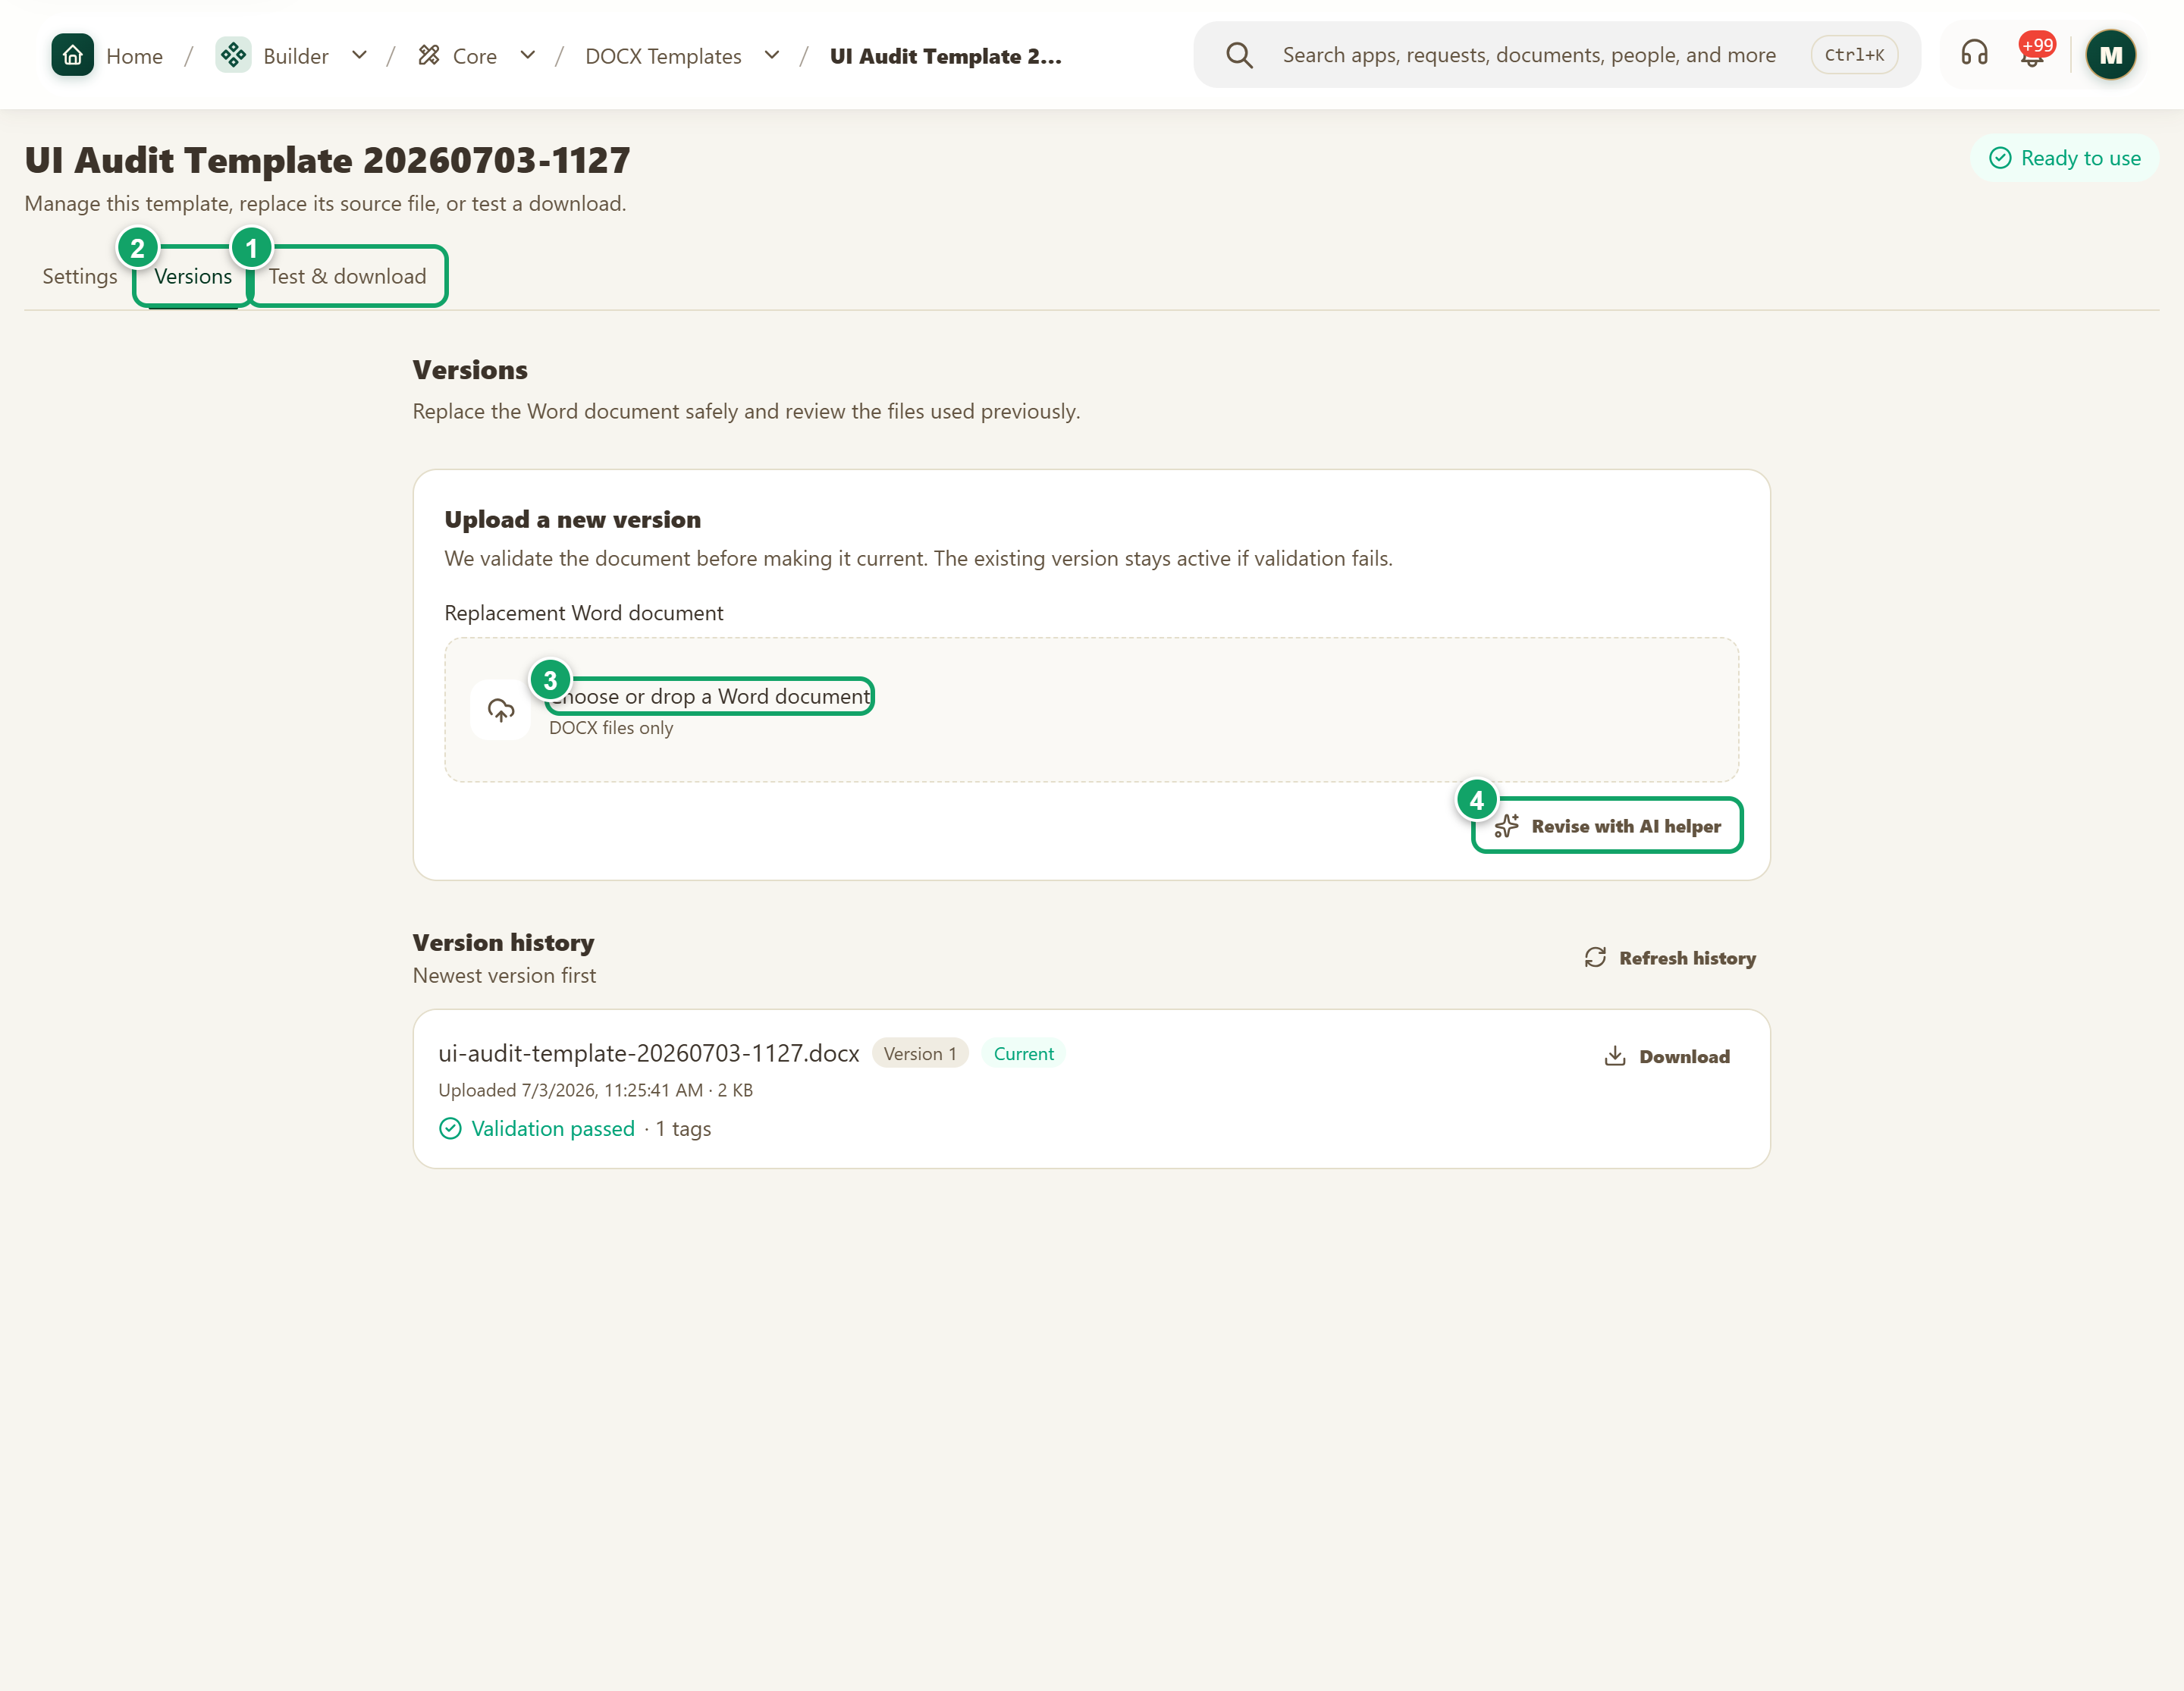
\includegraphics[width=0.95\linewidth,height=0.72\textheight,keepaspectratio]{figures/screens/ch06-docx-workspace-en.png}
\caption{The “Versions” tab in a DOCX template workspace}
\label{fig:builder-docx-workspace-screen}
\shotnote{The image shows a test DOCX template on test2 open on the “Versions” tab, with the “Version history” below it showing the current version and its validation result. This screen holds both ways to create a new version, uploading a replacement file or asking the helper for a draft, which is why testing comes first. ① “Test \& download”: try the template on a record before any change. ② “Versions”. ③ “Choose or drop a Word document”: pick the replacement file here. ④ “Revise with AI helper”: opens the helper page to choose the context and write the request.}
\end{figure}

\begin{table}[H]
\centering
\caption{Workspace tabs}
\label{tab:builder-docx-workspace-tabs}
\begin{tabularx}{\linewidth}{R{3.6cm} Y}
\rcHeaderRow
\thh{Tab} & \thh{Content and action}\\
Settings & “Template name”, “Description (optional)”, the downloaded file name and “Document permissions”, then “Save changes”.\\
Versions & Choose a replacement Word document and press “Validate and upload”; KayanOS validates the file before making it the current version. “Version history” lists versions newest first, with the “Current” mark, the validation result and a “Download” button.\\
Test \& download & Choose the test data: “Use a record” or “Paste JSON — Advanced”, then the Word or PDF format. “Advanced options” change the file name and permissions for this download only; then press “Render and download”.\\
\end{tabularx}
\end{table}

\begin{table}[H]
\centering
\caption{The DOCX AI helper}
\label{tab:builder-docx-workspace-ai}
\begin{tabularx}{\linewidth}{R{3.6cm} Y}
\rcHeaderRow
\thh{Stage} & \thh{What happens}\\
Start & From “Create with AI helper” when creating a template, or “Revise with AI helper” in “Versions” to revise the current version.\\
Context & Choose “Use entity context” with an optional record; without a record, sample data is used. Or choose “Manual JSON” within 256 KiB.\\
Consent to send & You confirm that the document text, the context and your instruction go to the AI provider your organization configured. The Word file itself is not sent.\\
Review & Every request creates a numbered revision: read the “Change summary” and “Template tags”, render a preview or press “Download DOCX”. Every item in “Questions to resolve” must be resolved before approval.\\
Approve or discard & “Approve and save” creates a new version without changing the template's settings or the actions linked to it; “Discard draft” removes it. A draft expires after 24 hours without activity, and after seven days at most.\\
\end{tabularx}
\end{table}

\begin{rcwarn}[A new version works immediately]
Action buttons on records always use the current version, so any version you upload or approve reaches users at once. Test the file on a real record before uploading it, and keep a copy of the approved file outside KayanOS.
\end{rcwarn}

\begin{figure}[H]
\centering
\begin{tikzpicture}[node distance=0.5cm]
\node[stepBox] (a) {Open the template};
\node[stepBox,below=of a] (b) {Test \& download on a record};
\node[stepBox,below=of b] (c) {New version: upload a file\\or a helper draft};
\node[stepBox,below=of c] (d) {Review and test};
\node[stepBox,below=of d] (e) {Becomes the current version};
\draw[flowsTo] (a) -- (b);
\draw[flowsTo] (b) -- (c);
\draw[flowsTo] (c) -- (d);
\draw[flowsTo] (d) -- (e);
\end{tikzpicture}
\rclegend
\caption{Changing a DOCX template safely}
\label{fig:builder-docx-workspace-flow}
\shotnote{The diagram brings together the two ways to create a new version: uploading a replacement file, or approving a draft the helper proposed. Either way, review comes before the version becomes current, because record actions use it from that moment on.}
\end{figure}

\subsection{Steps and check}
\begin{enumerate}
\item Open the template, then open “Test \& download”, choose “Use a record” and select a real record.
\item Choose the format, press “Render and download” and review the output file.
\item To change the wording by hand, open “Versions”, choose the replacement Word document, then press “Validate and upload”.
\item To change it with the helper, press “Revise with AI helper”, choose the context, write one focused request in “Instruction”, then confirm sending and press “Start AI helper”. Later requests go through the “Generate draft” button.
\item Review the “Change summary” and the preview, resolve open questions, then press “Approve and save”.
\end{enumerate}

\textbf{Check and recovery:} the message “A new template version is ready to use.” should appear, and the new version should carry the “Current” mark in “Version history”. If “This document was not uploaded” appears, press “View issues” and fix the file; the previous version stays active until then. If the helper button does not appear, ask an organization administrator to turn on “AI in builders”.

\clearpage
\section{XLSX Templates}
\label{sec:builder-feature-xlsx-templates}

An XLSX template is an Excel workbook with tags of the same kind, which KayanOS fills from the record's data and downloads as Excel or PDF. It suits lists and tabular reports with repeating rows, because tags can repeat rows and columns. A tag placed alone in a cell keeps the value's type as a number or date.

\textbf{Path and who uses it:} “Builder” → “Core” → “XLSX Templates”. Managed by those with Builder administration.

\begin{rcnote}[Example: Horizon]
The system administrator prepares a “Branch visits sheet” workbook that repeats a row for each visit, and links it to an action button of kind “XLSX template”, so Sarah Al-Khatib downloads the sheet ready in Excel. They upload the workbook from ①.
\end{rcnote}

\begin{figure}[H]
\centering
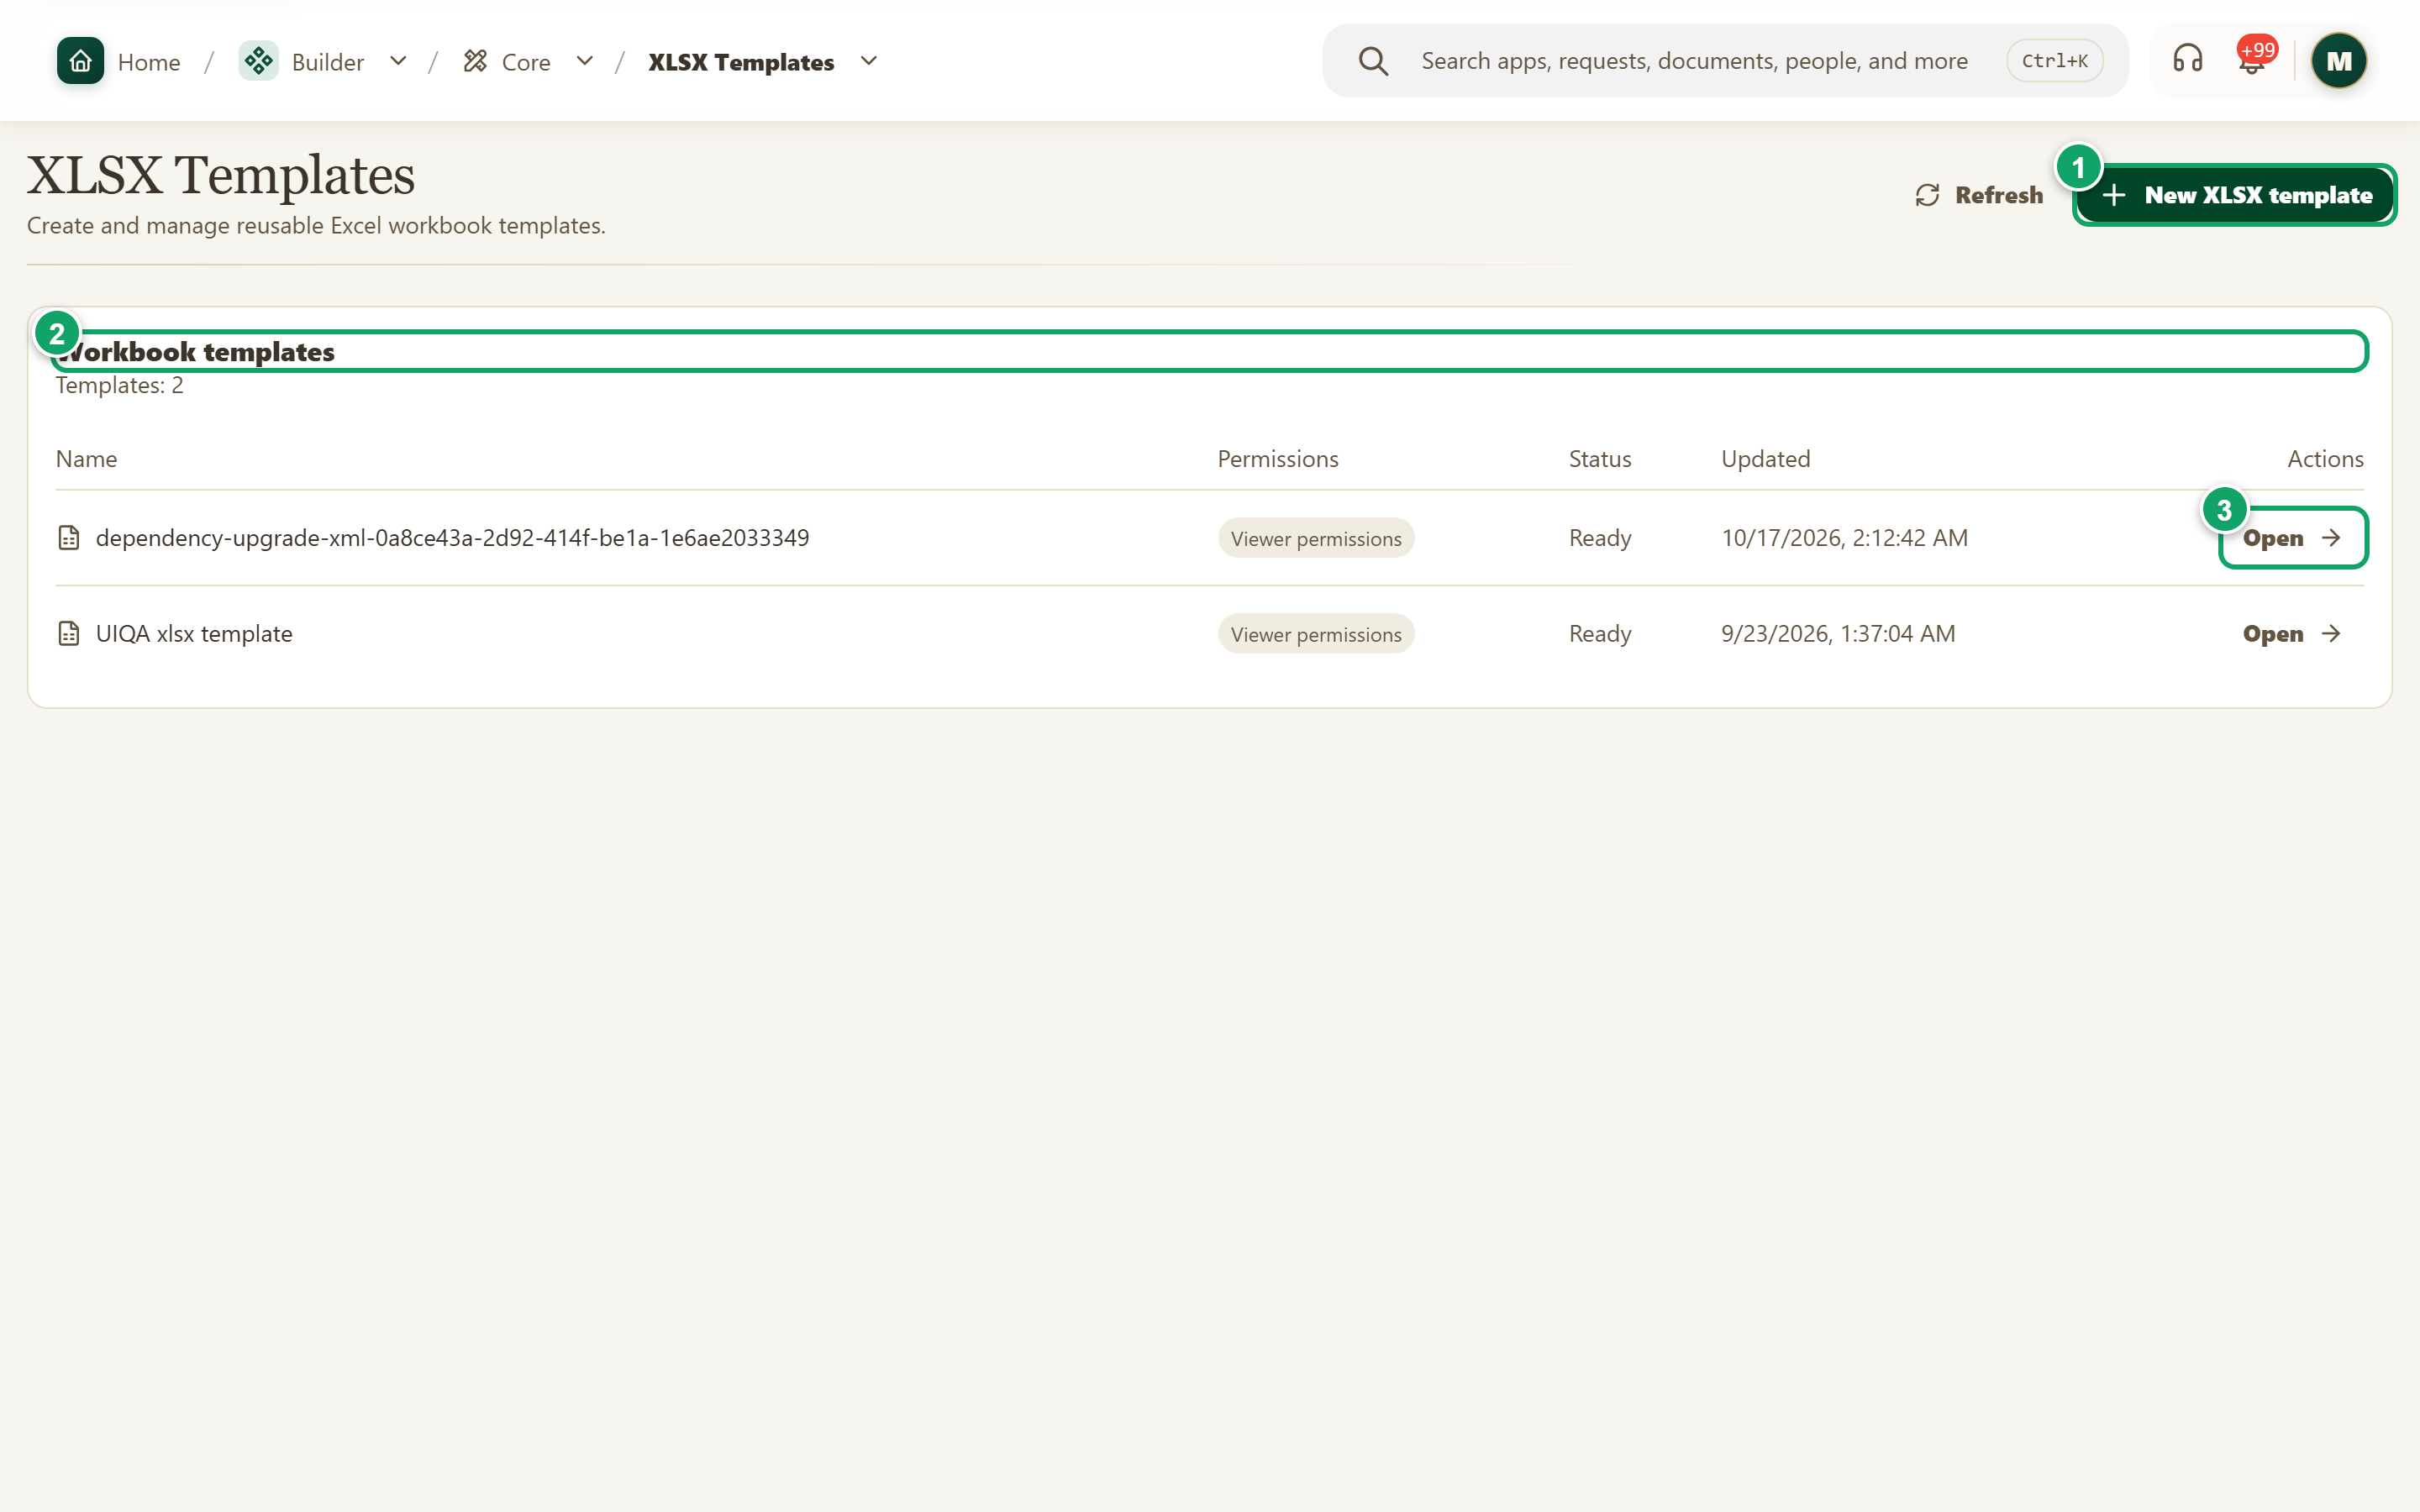
\includegraphics[width=0.95\linewidth,height=0.72\textheight,keepaspectratio]{figures/screens/ch06-xlsx-en.png}
\caption{The “XLSX Templates” page}
\label{fig:builder-xlsx-templates-screen}
\shotnote{The page lists workbook templates and their status, here test templates. ① “New XLSX template”. ② “Workbook templates”. ③ “Open”.}
\end{figure}


\begin{table}[H]
\centering
\caption{What do you find here?}
\label{tab:builder-xlsx-data}
\begin{tabularx}{\linewidth}{R{3.6cm} Y}
\rcHeaderRow
\thh{Part} & \thh{Content and action}\\
Workbook templates & The list of templates and their status: “Ready” or “Needs an Excel workbook”.\\
New XLSX template & Upload an “Excel workbook” and write the “Template name”; you can set the “Downloaded filename expression” and “Data permissions”.\\
Validation at upload & KayanOS rejects workbooks with macros, embedded objects or links to external workbooks, and lists the issues under “This workbook needs attention”.\\
Versions & Replace the workbook with a new version and review earlier versions.\\
Test \& download & Try the template with data, then “Render XLSX” or “Render PDF”.\\
\end{tabularx}
\end{table}

\begin{figure}[H]
\centering
\begin{tikzpicture}[node distance=0.5cm]
\node[entity] (tpl) {XLSX template};
\node[entityOpt,below right=0.7cm and 0.3cm of tpl] (xlsx) {Excel file};
\node[entityOpt,below left=0.7cm and 0.3cm of tpl] (pdf) {PDF file};
\draw[dependsOnOpt] (tpl.south) -- ++(0,-0.3) -| (xlsx.north);
\draw[dependsOnOpt] (tpl.south) -- ++(0,-0.3) -| (pdf.north);
\end{tikzpicture}
\rclegend
\caption{The two output formats}
\label{fig:builder-xlsx-outputs}
\shotnote{The figure shows that one template produces an Excel or PDF file, and you choose what is allowed when linking it to the action with “Allow PDF”. Use Excel when the recipient needs to work with the numbers, and PDF when you want a fixed copy to view or archive.}
\end{figure}

\subsection{Steps and check}
\begin{enumerate}
\item Prepare the workbook in Excel and place the tags in the right cells.
\item Open “XLSX Templates” and press “New XLSX template”, upload the workbook, write the name and press “Create template”.
\item Try the template from “Test \& download”, then add an action of kind “XLSX template” in the record type and choose the template.
\end{enumerate}

\textbf{Check and recovery:} the template's status should be “Ready”, and the row should repeat for each item in the output file. If a number shows as text, put the tag alone in its cell. If you cannot create the template, managing templates needs Builder administration, not only a full seat.

\clearpage
\section{XLSX tags and printing}
\label{sec:builder-feature-xlsx-tags}

Workbook tags are written in ordinary cells, and the main difference from Word is direction: the \en{each} tag repeats rows downward, and the \en{eachCol} tag repeats columns sideways. When a row loop crosses a column loop, a full grid results, with a row for each item of the first list and a column for each item of the second. KayanOS keeps the formulas, formatting, charts and print settings in the workbook, and updates their references when rows and columns expand.

\textbf{Path and who uses it:} tags are written in Excel before uploading the workbook from “Builder” → “Core” → “XLSX Templates”. They are written by template managers.

\begin{rcnote}[Example: Horizon]
In the “Branch visits sheet”, the system administrator places a row loop for each branch and a column loop for each month. The output has a row for Head Office Damascus and one for the Aleppo Branch, and each cell holds the branch's number of visits that month.
\end{rcnote}

\begin{table}[H]
\centering
\caption{Cell tags and loops}
\label{tab:builder-xlsx-tags-loops}
\begin{tabularx}{\linewidth}{R{3.6cm} Y}
\rcHeaderRow
\thh{Tag} & \thh{What it does and where it goes}\\
\en{\{\{ \$record.field\_key \}\}} & Alone in a cell, it stays a number, a Boolean or a blank cell; next to other text, it becomes text. Text starting with \en{=}, \en{+}, \en{-} or \en{@} stays text and never becomes a formula.\\
\en{\{\{\#each list as item\}\}} and \en{\{\{/each\}\}} & Repeat the body rows between them. Each sits in its own row with no other non-empty cell.\\
\en{\{\{\#if ...\}\}}, \en{\{\{else\}\}} and \en{\{\{/if\}\}} & Choose rows by a condition, each in its own row in the same way.\\
\en{\{\{\#eachCol list as item\}\}} and \en{\{\{/eachCol\}\}} & Repeat the columns between them. Each sits in its own column with no other non-empty cell.\\
\en{\{\{\#ifCol ...\}\}}, \en{\{\{elseCol\}\}} and \en{\{\{/ifCol\}\}} & Choose columns by a condition, each in its own marker column.\\
\end{tabularx}
\end{table}

\begin{table}[H]
\centering
\caption{Directives, formulas and printing}
\label{tab:builder-xlsx-tags-directives}
\begin{tabularx}{\linewidth}{R{3.6cm} Y}
\rcHeaderRow
\thh{Item} & \thh{What you need to know}\\
\en{\{\{@hideRow ...\}\}} and \en{\{\{@hideColumn ...\}\}} & Hide the output row or column when the expression is true.\\
\en{\{\{@link url label\}\}} & A safe link starting with \en{http}, \en{https} or \en{mailto}.\\
\en{\{\{@image ... width=120\}\}} and \en{\{\{@qr ... width=120\}\}} & An image or QR code that takes a whole cell and moves with expanded rows and columns.\\
Formulas & Formulas stay as they are and their references are updated, respecting fixed references such as \en{\$A1} and \en{A\$1}. KayanOS does not calculate formulas itself; it asks Excel to recalculate when the file opens.\\
Print setup & Orientation, margins, print area, fit to width and repeated titles are set in the source workbook, because PDF conversion uses them as they are.\\
\end{tabularx}
\end{table}

\begin{rcwarn}[A marker row or column shares nothing]
If a heading or formula is placed in a loop's marker row or column, validation rejects the workbook. Two loops in the same direction that cross without one fully containing the other are rejected too.
\end{rcwarn}

\begin{figure}[H]
\centering
\begin{tikzpicture}[node distance=0.5cm]
\node[stepBox] (a) {Separate marker rows and columns};
\node[stepBox,below=of a] (b) {Print setup in the workbook};
\node[stepBox,below=of b] (c) {Upload and validation};
\node[stepBox,below=of c] (d) {Review the Excel file};
\node[stepBox,below=of d] (e) {Review the PDF file};
\draw[flowsTo] (a) -- (b);
\draw[flowsTo] (b) -- (c);
\draw[flowsTo] (c) -- (d);
\draw[flowsTo] (d) -- (e);
\end{tikzpicture}
\rclegend
\caption{From the source workbook to a printable file}
\label{fig:builder-xlsx-tags-flow}
\shotnote{The diagram puts print setup before upload because the PDF is produced from the workbook itself and adds no settings of its own. It separates reviewing the Excel file, to check formulas and rows, from reviewing the PDF, to check pages and right-to-left direction.}
\end{figure}

\subsection{Steps and check}
\begin{enumerate}
\item In the workbook, add a marker row for the start of the loop, then the body row, then a marker row for the end, leaving the other cells of both marker rows empty.
\item If the list runs sideways, use \en{eachCol} in two separate columns on either side of the body column.
\item Put each numeric value alone in its cell, and write formulas with the references you want fixed.
\item In Excel, set the page orientation, print area and fit to width, then save the file as \en{.xlsx}.
\item Upload the workbook, then test it with an empty list, one item and several items.
\end{enumerate}

\textbf{Check and recovery:} the row or column should repeat once per item, and formulas should point to the expanded range. If \en{ROW\_MARKER\_NOT\_EXCLUSIVE} or \en{COLUMN\_MARKER\_NOT\_EXCLUSIVE} appears, clear everything else from the marker row or column. If a list repeats downward instead of sideways, replace \en{each} with \en{eachCol}. If columns are cut off in the PDF, make the page landscape and set fit to width.

\clearpage
\section{XLSX workspace}
\label{sec:builder-feature-xlsx-workspace}

When you open an XLSX template, its workspace appears with three tabs: “Settings”, “Versions” and “Test \& download”. A badge in its header shows “Ready to use” or “Needs an XLSX version”. Here you edit the template's details, replace the workbook with a new version after it is validated, and try the output before linking it to an action. When “AI in builders” is on, an “AI workbook helper” button appears; it proposes changes to the workbook in a draft that you review.

\textbf{Path and who uses it:} “Builder” → “Core” → “XLSX Templates” → “Open”. Used by template managers.

\begin{rcnote}[Example: Horizon]
The system administrator adds a visit notes column to the “Branch visits sheet” and uploads the new workbook from “Versions”. They test it in “Test \& download” with data for two visits and press “Render PDF” to make sure the sheet fits on one page. They upload the workbook from ①, write the two visits in ③ and press ⑤.
\end{rcnote}

\begin{figure}[H]
\centering
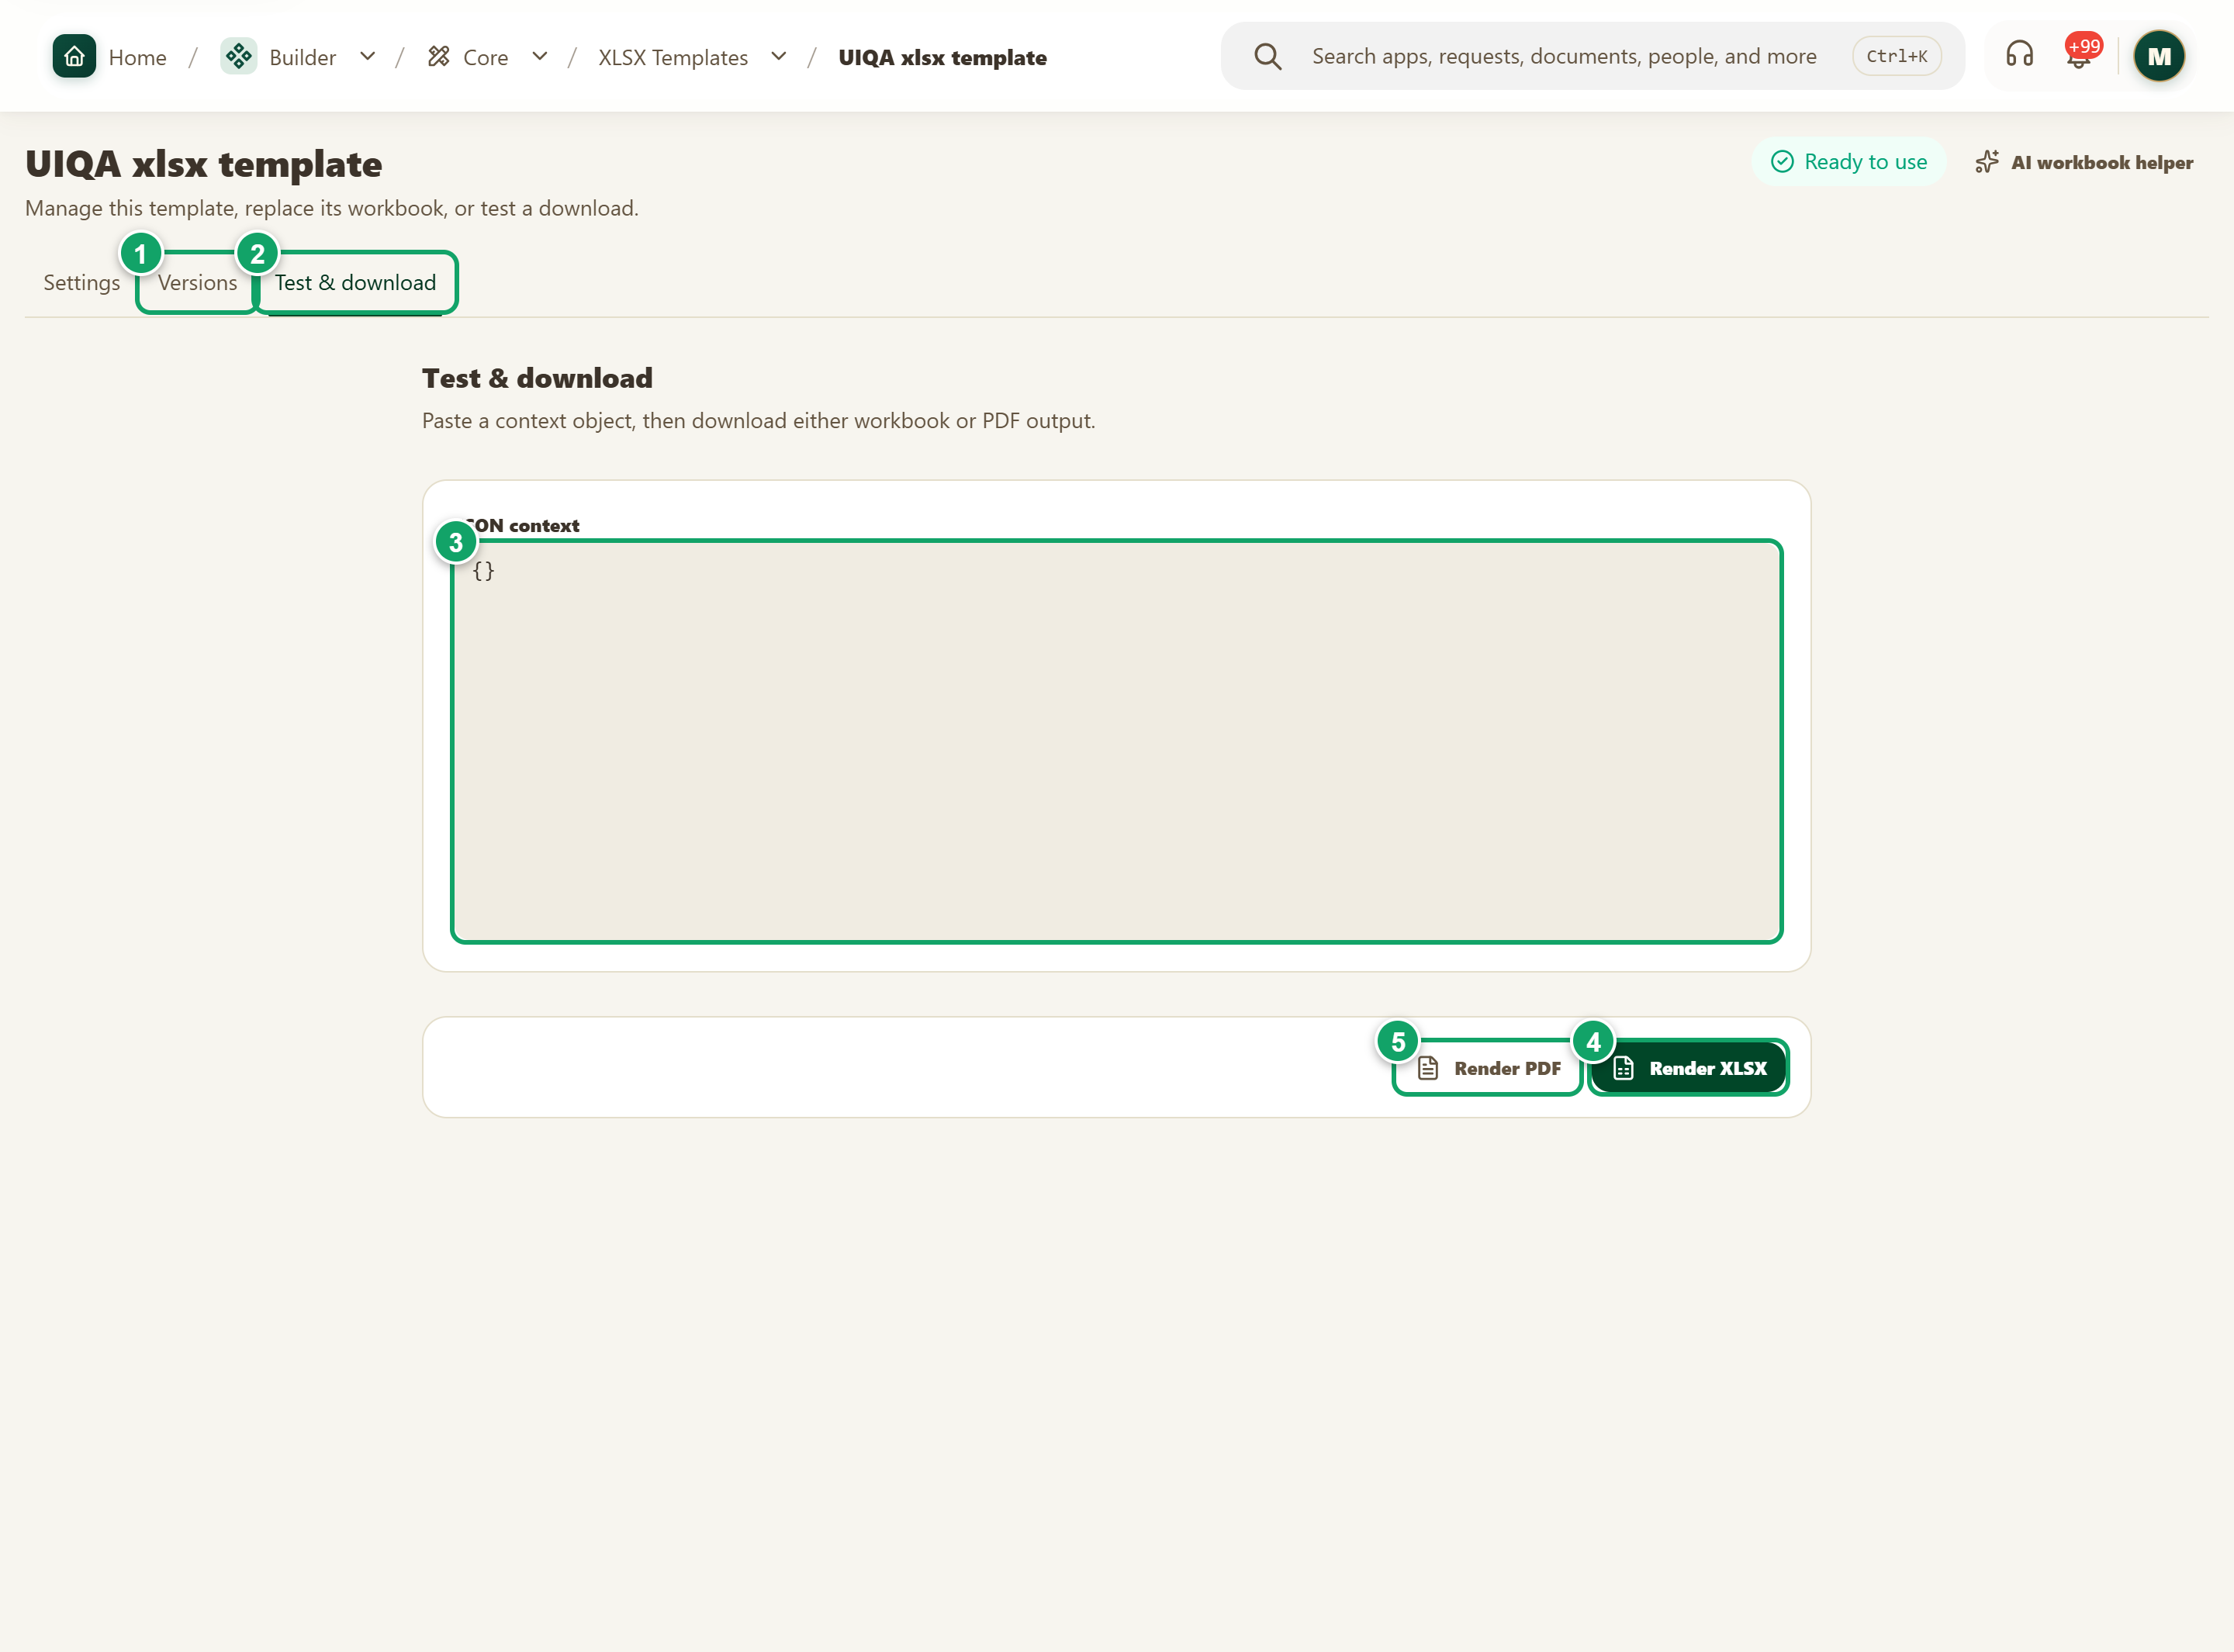
\includegraphics[width=0.95\linewidth,height=0.72\textheight,keepaspectratio]{figures/screens/ch06-xlsx-workspace-en.png}
\caption{The “Test \& download” tab in an XLSX template workspace}
\label{fig:builder-xlsx-workspace-screen}
\shotnote{The image shows a test XLSX template on test2 open on “Test \& download”, with the context box holding only empty braces. It shows that testing a workbook relies on data you write yourself as JSON, not on a record you pick as in DOCX templates. ① “Versions”: upload the replacement workbook here. ② “Test \& download”. ③ “JSON context”: write an object holding \en{\$record} and its fields. ④ “Render XLSX”: downloads the Excel file to review rows and formulas. ⑤ “Render PDF”: downloads the PDF to review the pages.}
\end{figure}

\begin{table}[H]
\centering
\caption{Workspace tabs}
\label{tab:builder-xlsx-workspace-tabs}
\begin{tabularx}{\linewidth}{R{3.6cm} Y}
\rcHeaderRow
\thh{Tab} & \thh{Content and action}\\
Settings & “Template name”, “Description”, “Downloaded filename expression” and “Data permissions”, then “Save settings”.\\
Versions & In “Replace workbook”, choose a file and press “Validate and upload”; it becomes current only if validation succeeds, otherwise “This workbook was not uploaded” appears. “Version history” lists versions newest first with the “Current” mark.\\
Test \& download & Write the test data in “JSON context”, then press “Render XLSX” or “Render PDF” to download the file.\\
Workbook helper & Write “Instructions” describing the change, confirm that the workbook context is sent to the AI provider, then press “Generate draft”. Review it with “Download preview XLSX” and “Review PDF”, then press “Approve version” and “Confirm approval”, or “Discard draft”.\\
\end{tabularx}
\end{table}

\begin{table}[H]
\centering
\caption{What do you review in the output?}
\label{tab:builder-xlsx-workspace-checks}
\begin{tabularx}{\linewidth}{R{3.6cm} Y}
\rcHeaderRow
\thh{Review} & \thh{Expected result}\\
Row and column count & Equal to the number of items, with row formatting and column width kept.\\
Types & Numbers stay numbers, and Booleans stay Booleans.\\
Formulas and charts & They point to the expanded range, and show correct values after the file opens.\\
PDF file & Print area, margins, orientation, page breaks and Arabic text are correct.\\
\end{tabularx}
\end{table}

\begin{rcwarn}[The helper never overwrites a newer change]
For each change, the helper names the sheet, the cell and its expected content. If the workbook changed after the proposal, approval fails instead of overwriting the newer cell. Approval also does not work until the data-mapping questions the helper asks are resolved.
\end{rcwarn}

\begin{figure}[H]
\centering
\begin{tikzpicture}[node distance=0.5cm]
\node[stepBox] (a) {Open the template};
\node[stepBox,below=of a] (b) {Replace the workbook or\\a helper draft};
\node[stepBox,below=of b] (c) {Workbook validation};
\node[stepBox,below=of c] (d) {Test with a JSON context};
\node[stepBox,below=of d] (e) {Review XLSX and PDF};
\draw[flowsTo] (a) -- (b);
\draw[flowsTo] (b) -- (c);
\draw[flowsTo] (c) -- (d);
\draw[flowsTo] (d) -- (e);
\end{tikzpicture}
\rclegend
\caption{The XLSX template update cycle}
\label{fig:builder-xlsx-workspace-flow}
\shotnote{The diagram shows that every new version passes validation before it becomes current, whether you upload it yourself or approve it from the helper. Testing in both formats follows, because a working Excel file does not mean the PDF conversion service produced correct pages.}
\end{figure}

\subsection{Steps and check}
\begin{enumerate}
\item Open the template, change what you need in “Settings”, then press “Save settings”.
\item To replace the workbook, open “Versions”, choose the new file in “Replace workbook”, then press “Validate and upload”.
\item Open “Test \& download” and write in “JSON context” an object holding \en{\$record} and its fields, such as \en{\{"\$record": \{"total": 12\}\}}.
\item Press “Render XLSX” and review rows and formulas, then press “Render PDF” and review the pages.
\end{enumerate}

\textbf{Check and recovery:} the message “XLSX version uploaded.” should appear, and the new version should carry the “Current” mark. If “Enter a valid JSON object.” appears, make sure the text starts and ends with a curly brace. If Excel works but PDF fails, the problem is the conversion service, not the template, so ask the system administrator to check it.

\clearpage
\section{Print templates}
\label{sec:builder-feature-print-templates}

A print template is a document you design inside KayanOS by drag and drop, without uploading a Word file. It prints a form's requests or a record type's records as PDF or Word, on the organization's letterhead and identity. The “Print templates” page lists every existing template and its status; you create a new one from inside the form or record-type builder by pressing “Print”.

\textbf{Path and who uses it:} “Builder” → “Core” → “Print templates”. Used by those who build forms and record types.

\begin{rcnote}[Example: Horizon]
The system administrator opens the “Visit requests” type, presses “Print” and chooses “Start from this record type” to design a visit sheet with a verification QR code, then publishes it so it appears under “Print” on every request. They reach the template from ③.
\end{rcnote}

\begin{figure}[H]
\centering
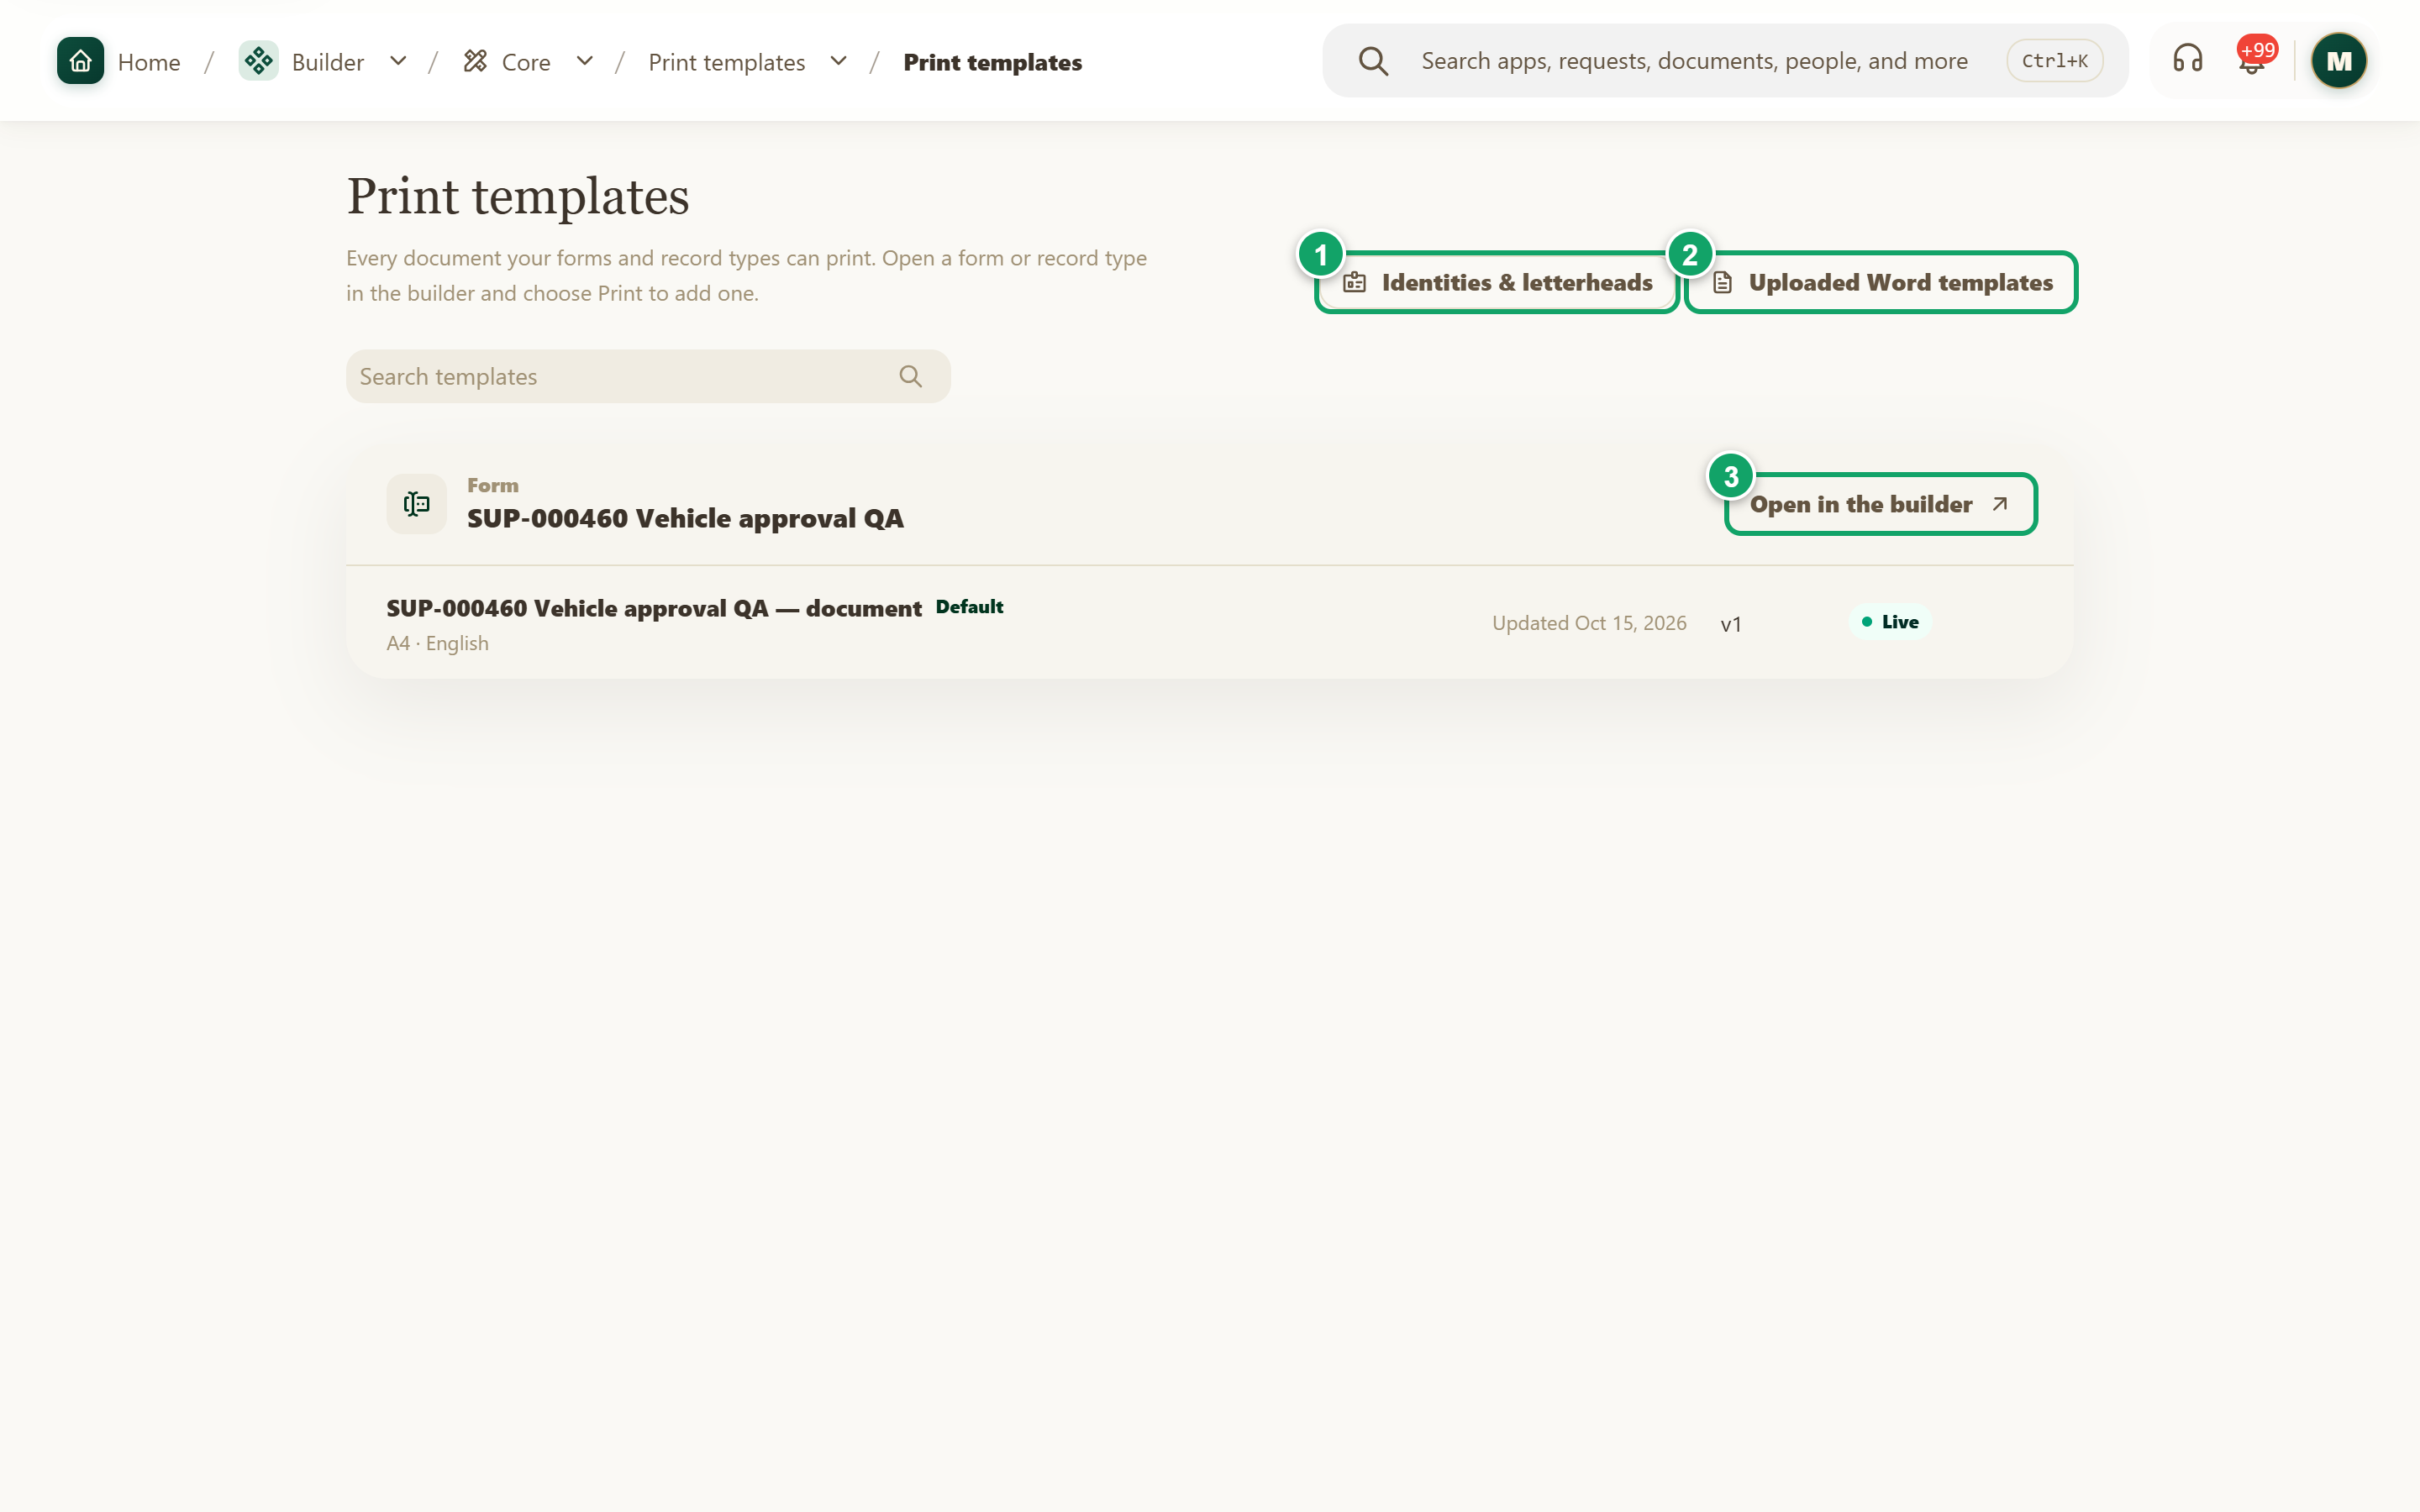
\includegraphics[width=0.95\linewidth,height=0.72\textheight,keepaspectratio]{figures/screens/ch06-print-en.png}
\caption{The “Print templates” library}
\label{fig:builder-print-templates-screen}
\shotnote{The page lists print templates grouped by form or record type, with their status. The template shown is a test template. ① “Identities \& letterheads”. ② “Uploaded Word templates”. ③ “Open in the builder”: opens the form or type where the template is edited.}
\end{figure}


\begin{table}[H]
\centering
\caption{What do you find here?}
\label{tab:builder-print-data}
\begin{tabularx}{\linewidth}{R{3.6cm} Y}
\rcHeaderRow
\thh{Part} & \thh{Content and action}\\
Template library & Templates grouped by form or record type, with paper size, language, version and status: “Live”, “Draft” or “Unpublished changes”, plus “Open in the builder”.\\
The “Print templates” sheet & Opens from the “Print” button in the form or type builder and shows for each template “Printed from”: “Print menu”, “Bulk print” or “Not offered until published”. It offers “Open”, “Make default” and “Archive”.\\
New template & From the same sheet: “Start from this form”, “Start from this record type” or “Blank page on the org letterhead”.\\
Output & Formats people can download, the file name, “Who can print”, keeping a copy on the record, and a verification page opened by the QR code.\\
\end{tabularx}
\end{table}

\begin{figure}[H]
\centering
\begin{tikzpicture}[node distance=0.5cm]
\node[stepBox] (a) {Print from the form or type builder};
\node[stepBox,below=of a] (b) {Design data and blocks};
\node[stepBox,below=of b] (c) {Preview with a record};
\node[stepBox,below=of c] (d) {Publish};
\node[stepBox,below=of d] (e) {Print button on the record};
\draw[flowsTo] (a) -- (b);
\draw[flowsTo] (b) -- (c);
\draw[flowsTo] (c) -- (d);
\draw[flowsTo] (d) -- (e);
\end{tikzpicture}
\rclegend
\caption{From design to the print button}
\label{fig:builder-print-flow}
\shotnote{The diagram shows that a template is born inside the form or record-type builder, not on the library page, and is not offered to users before it is published. Previewing with a real record comes before publishing to catch empty fields or long tables before anyone prints them.}
\end{figure}

\subsection{Steps and check}
\begin{enumerate}
\item Open the form or record type in the builder, press “Print”, then choose a starting point.
\item Add fields and blocks, and set the paper, identity and letterhead under “Page”.
\item Press “Preview with a record” and “Download test PDF”, then set “Who can print” and press “Publish”.
\end{enumerate}

\textbf{Check and recovery:} the template should show as “Live” in the library and appear in “Choose a document” when pressing “Print” on a record. If it does not, make sure it is published, because a template is “Not offered until published”; use “Check against all records” to find records missing data.

\clearpage
\section{Print template builder: data and blocks}
\label{sec:builder-feature-print-builder}

The builder opens when you choose a starting point for a new template or press “Open” next to an existing one. The page appears in the middle as it will print, with three tabs beside it: “Data”, “Blocks” and “Page”, and on the other side the “Settings” for whatever you select on the page. The builder saves your work automatically, showing “Saving…” then “Saved”, but changes stay a draft that nobody sees until you publish. Every block on the page is real text in the PDF that can be selected and searched, not a picture of the page.

\textbf{Path and who uses it:} the form or record-type builder → “Print” → a starting point or “Open”. Used by whoever builds the form or record type.

\begin{rcnote}[Example: Horizon]
The system administrator drags the visit date field from the “This record” group onto the visit sheet and sets its “When it’s empty” option to “Stop print”. Then they add a “Show when” block around the review notes paragraph, so it prints only if Sarah Al-Khatib wrote a note. They take the field from ①, and the “Show when” block from ② and then ③.
\end{rcnote}

\begin{figure}[H]
\centering
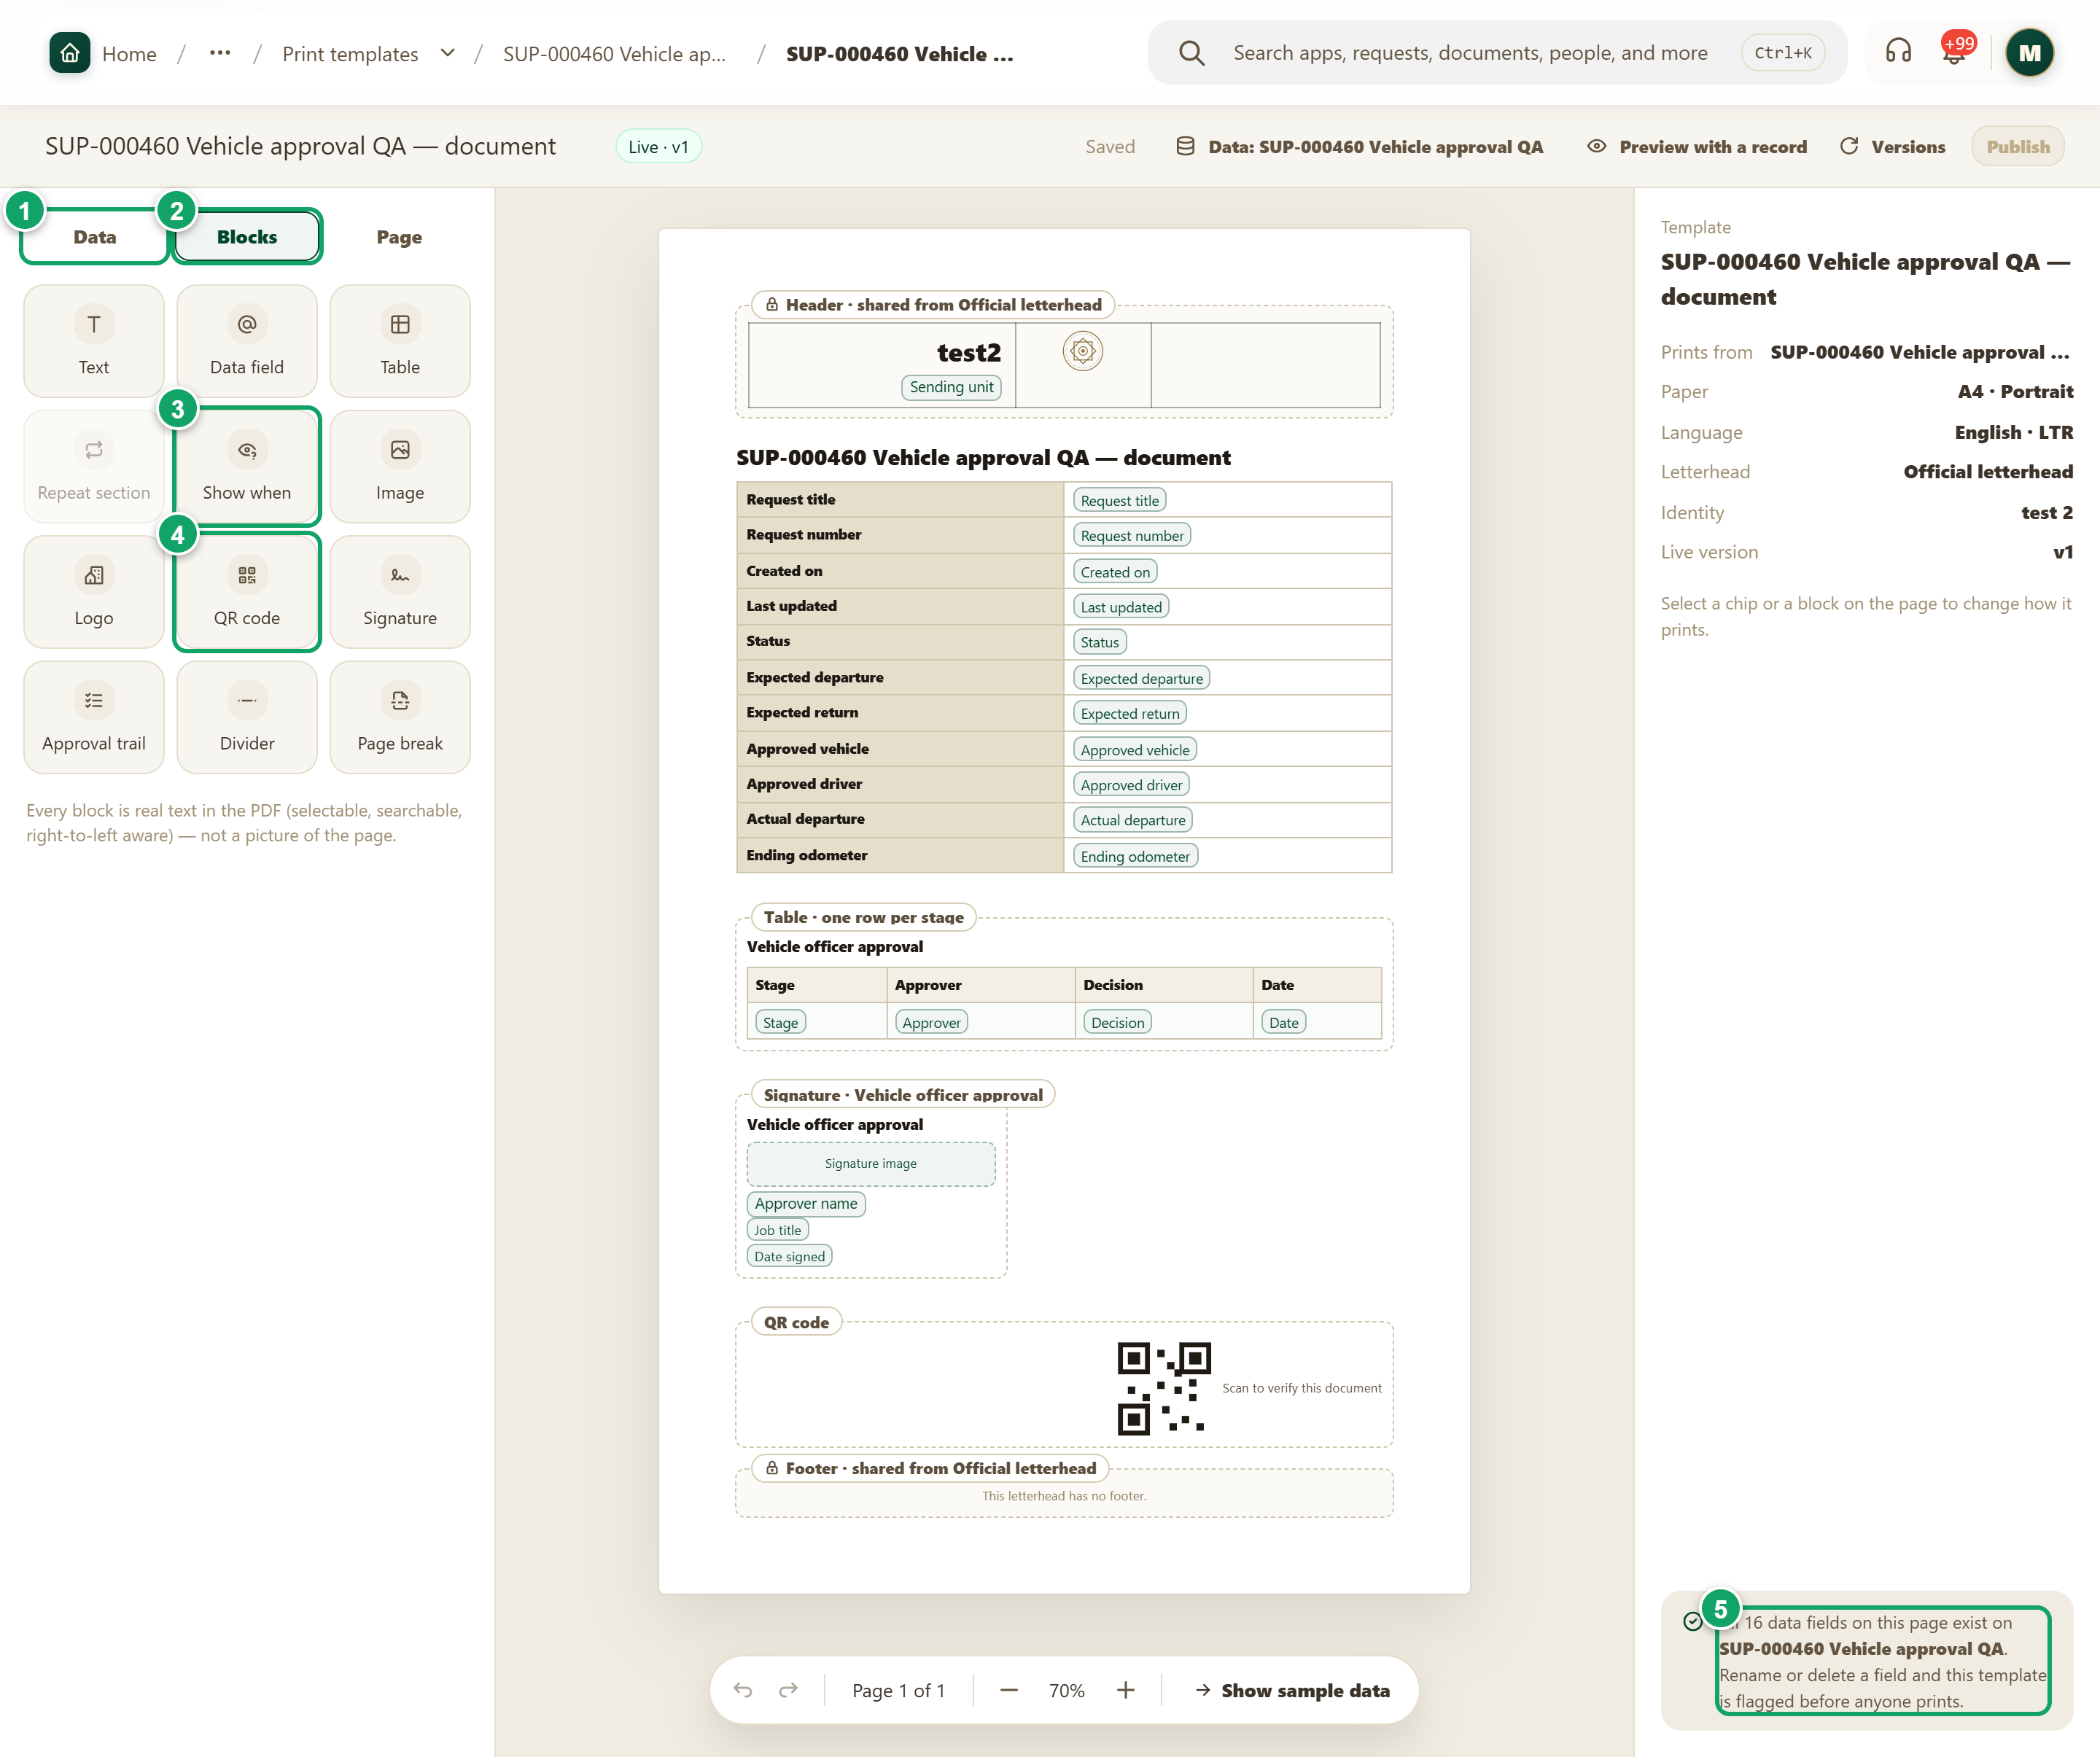
\includegraphics[width=0.95\linewidth,height=0.72\textheight,keepaspectratio]{figures/screens/ch06-print-builder-en.png}
\caption{The print template builder with the “Blocks” tab open}
\label{fig:builder-print-builder-screen}
\shotnote{The image shows a test print template for a form on test2 inside the builder, with the page in the middle as it will print, including its fields, the approvals table, the signature and the QR code. “Repeat section” is greyed out because this form has no lists, and the block only works with a list. ① “Data”: the fields you drag onto the page. ② “Blocks”. ③ “Show when”: a part that prints only when its conditions hold. ④ “QR code”: a code that opens the verification page. ⑤ The status bar: confirms that all data fields on the page still exist.}
\end{figure}

\begin{table}[H]
\centering
\caption{The “Data” tab}
\label{tab:builder-print-builder-data}
\begin{tabularx}{\linewidth}{R{3.6cm} Y}
\rcHeaderRow
\thh{Group} & \thh{What it holds}\\
“This request” or “This record” & The fields of the request or record being printed, each with its type, such as text, date or option.\\
“Linked records” & The fields of records this record links to; open them by pressing the record's name.\\
“Lists” & The lists that suit a “Repeat section” block, such as table answers and linked records.\\
“Approvals \& signatures” & Approval stages and who signed them, when the form or type has approvals.\\
“Organization” and “Document” & The identity's official details, and document data such as the date, page number and verification QR.\\
\end{tabularx}
\end{table}

You add a field by dragging it onto the page, or by typing \en{/} while writing and then choosing the field. Only fields you can read appear in the list.

\begin{table}[H]
\centering
\caption{The “Blocks” tab}
\label{tab:builder-print-builder-blocks}
\begin{tabularx}{\linewidth}{R{3.6cm} Y}
\rcHeaderRow
\thh{Block} & \thh{What it adds}\\
“Text” and “Data field” & A new paragraph, or a field you pick from the “Data” tab.\\
“Table” & A fixed table for layout.\\
“Repeat section” & A table with one row for each item of a list; you set its columns, title and what shows when the list is empty.\\
“Show when” & A part that prints only when all its conditions hold, using the same condition builder as form rules.\\
“Image” and “Logo” & An image from an image field of the request, or the logo of the identity the template prints under.\\
“QR code” & A code that opens the document's verification page when scanned.\\
“Signature” and “Approval trail” & A signature block for an approval stage showing the image, name, job title and date, or a table of the approval's stages.\\
“Divider” and “Page break” & A horizontal line, or the start of a new page.\\
\end{tabularx}
\end{table}

\subsection{Data field settings}

When you select a field on the page, its settings appear. For a date you choose the “Calendar”: “Gregorian”, “Hijri” or “Both”, then the “Format”. For a number you choose, for example, “Grouped (1,250)” or “Money”. “When it’s empty” sets what happens to an empty field: “Show —”, “Hide line” or “Stop print”; the last option blocks printing and tells the person which field to fill.

\begin{figure}[H]
\centering
\begin{tikzpicture}[node distance=0.5cm]
\node[stepBox] (a) {Choose a starting point};
\node[stepBox,below=of a] (b) {Drag fields from Data};
\node[stepBox,below=of b] (c) {Add blocks};
\node[stepBox,below=of c] (d) {Set each field's settings};
\node[stepBox,below=of d] (e) {Automatic save to the draft};
\draw[flowsTo] (a) -- (b);
\draw[flowsTo] (b) -- (c);
\draw[flowsTo] (c) -- (d);
\draw[flowsTo] (d) -- (e);
\end{tikzpicture}
\rclegend
\caption{Designing a print template's content}
\label{fig:builder-print-builder-flow}
\shotnote{The diagram orders the work from content to detail: fields first, then the blocks that organize them, then how each field prints. It ends with the draft because automatic saving is not publishing, so users see no change until you publish the template.}
\end{figure}

\subsection{Steps and check}
\begin{enumerate}
\item Open the form or record type in the builder, press “Print”, then choose a starting point or press “Open” next to a template.
\item Open “Data” and drag fields into place, or type \en{/} while writing to insert a field.
\item Open “Blocks” and add what you need, such as a “Repeat section” for a list or a “QR code” for verification.
\item Select each important field and set its format and what happens when it is empty.
\item Read the status bar under the page and make sure all data fields exist.
\end{enumerate}

\textbf{Check and recovery:} “Saved” should show in the builder header, and the status bar should say that the data fields on this page exist. If “A data field no longer exists” appears, the field was deleted or renamed and will print as —, so pick another field or remove it. If “Couldn’t save” appears, press “Try again”.

\clearpage
\section{Print template page settings}
\label{sec:builder-feature-print-page}

The “Page” tab sets the sheet a template prints on: its size, orientation, language and margins, the identity whose logo it carries, and the letterhead shown in its header and footer. It can also print a watermark on the document until the request is approved. These settings apply to this template only, so another template may use different paper or a different letterhead.

\textbf{Path and who uses it:} the print template builder → “Page”. Used by whoever designs the template.

\begin{rcnote}[Example: Horizon]
For the visit sheet, the system administrator chooses portrait A4 paper in Arabic, and the Horizon letterhead whose header shows on the first page only. They turn on the “Draft” watermark until the request reaches an approved status, so no unapproved sheet leaves without that mark. They set the paper in ② and ③, and choose the letterhead under ⑤.
\end{rcnote}

\begin{figure}[H]
\centering
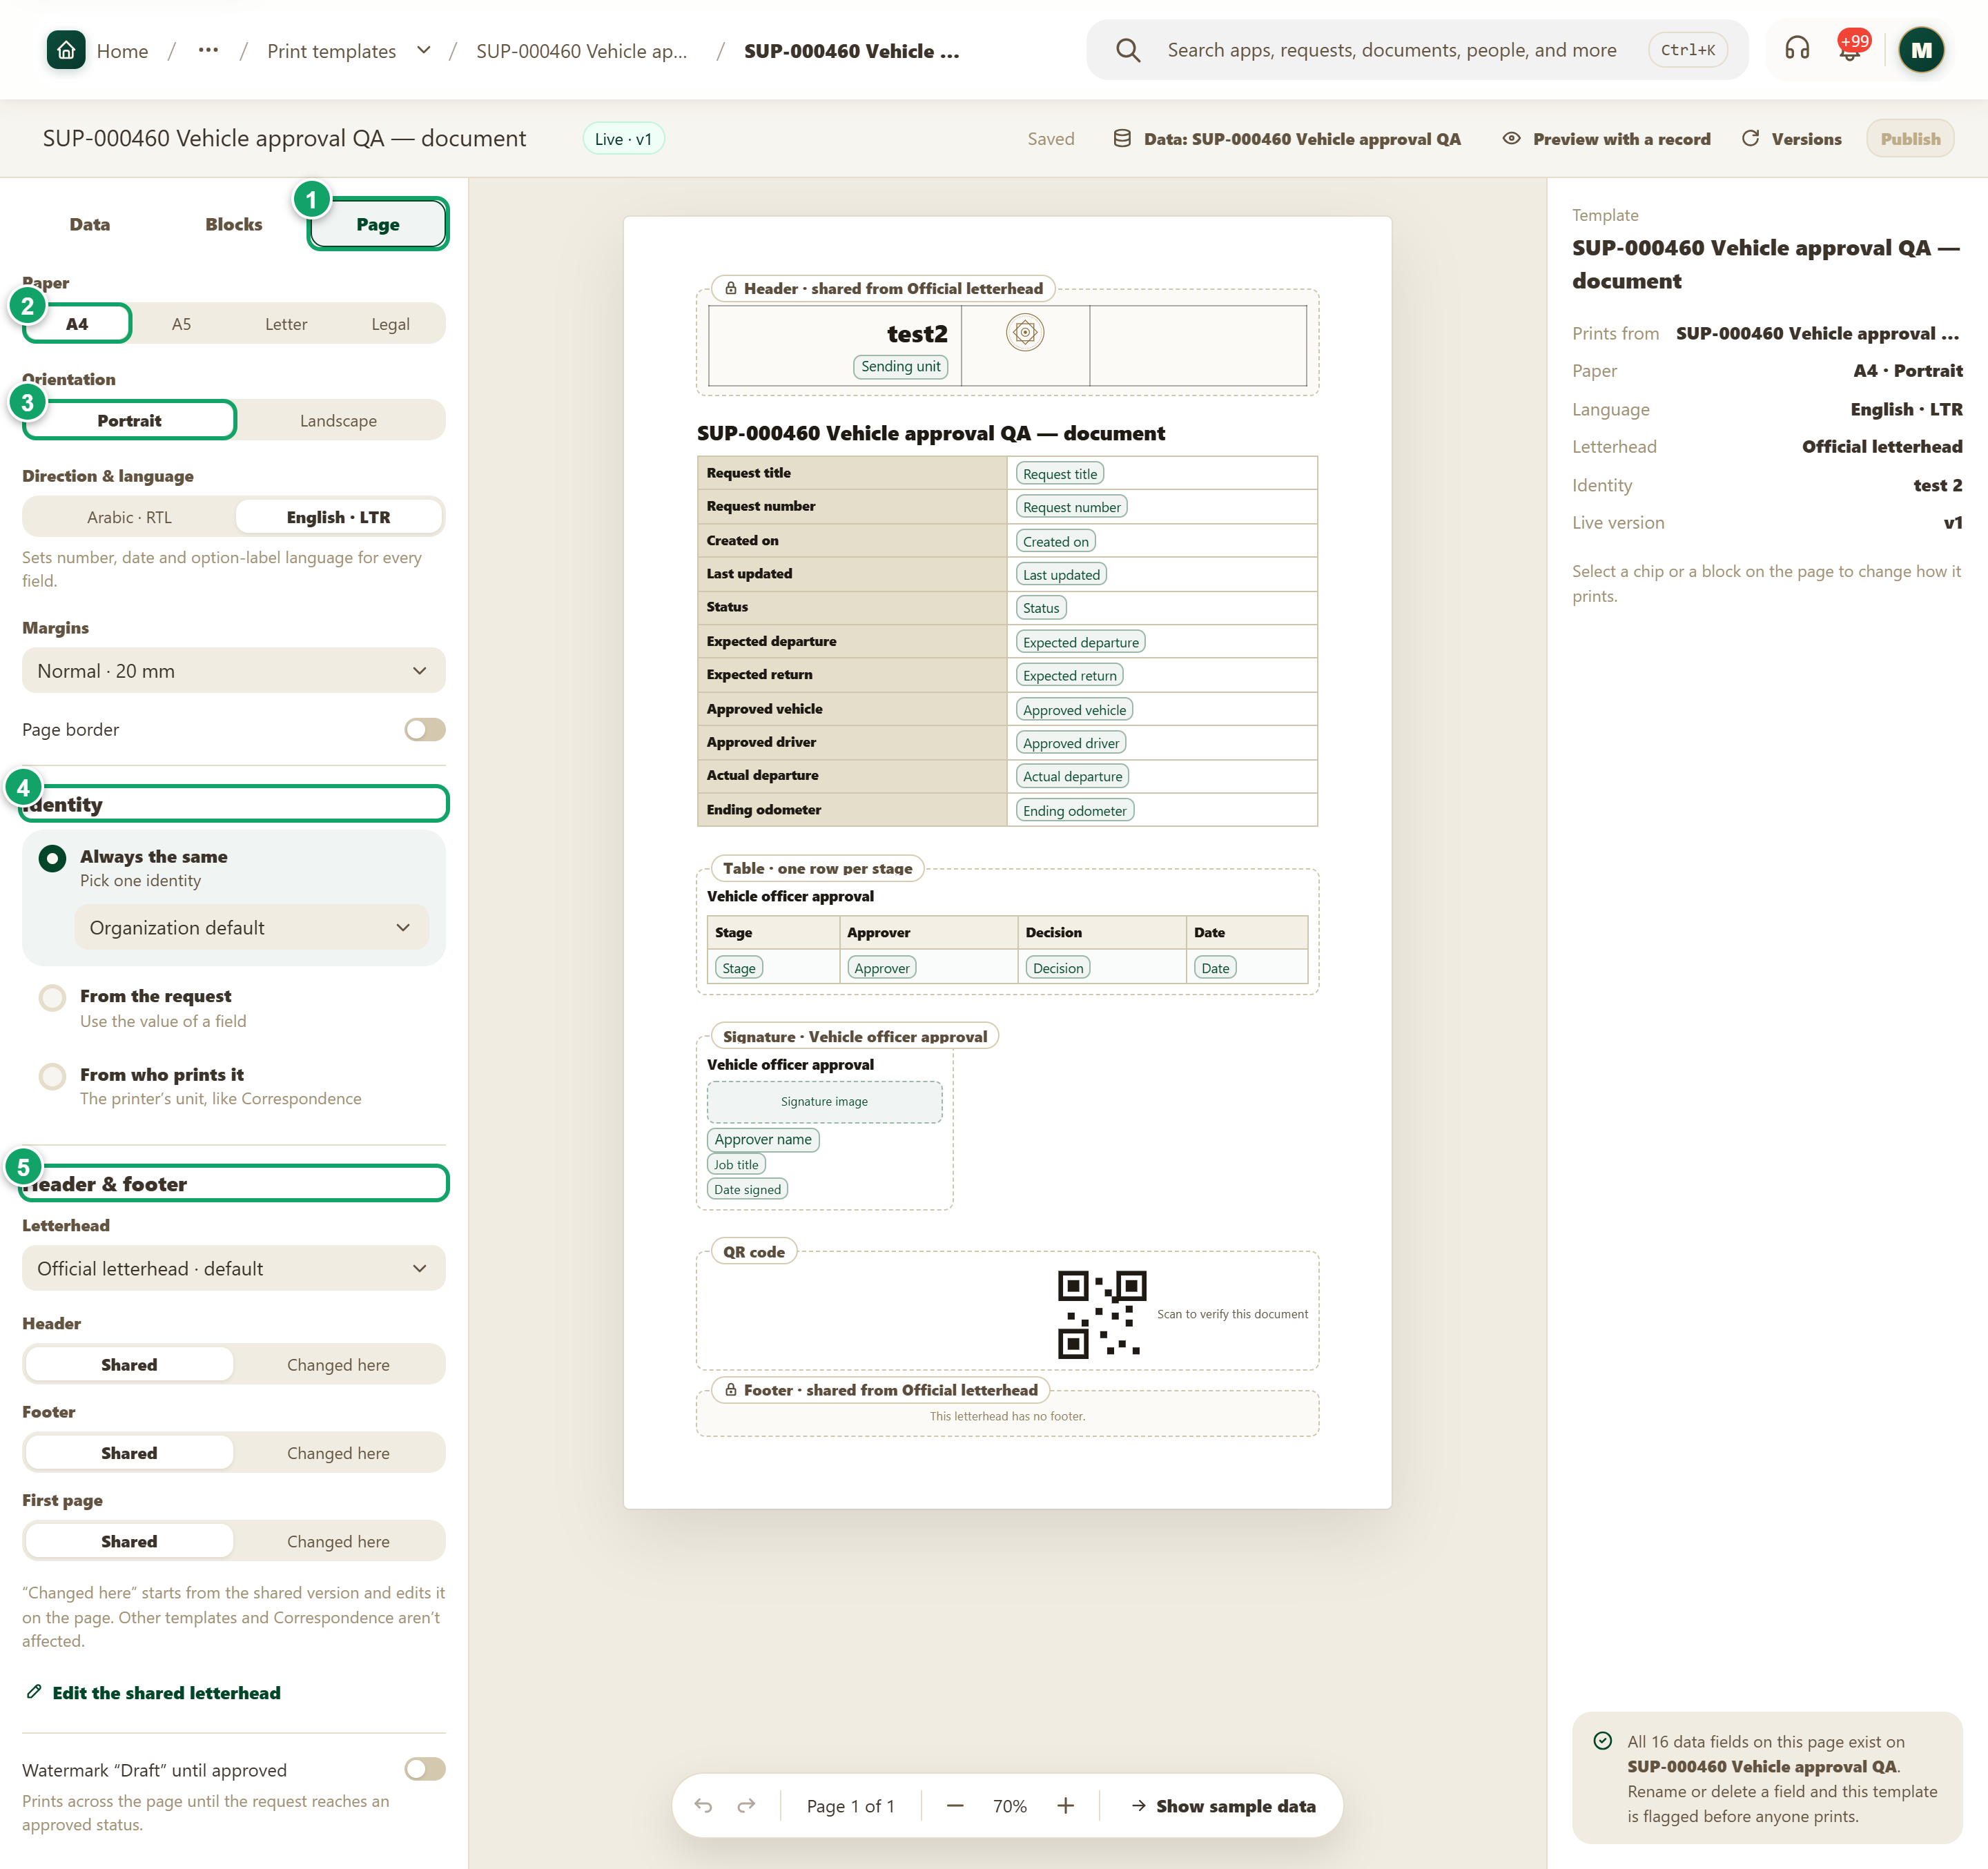
\includegraphics[width=0.95\linewidth,height=0.72\textheight,keepaspectratio]{figures/screens/ch06-print-page-en.png}
\caption{The “Page” tab in the print template builder}
\label{fig:builder-print-page-screen}
\shotnote{The image shows the page settings of the same test template: portrait A4 paper, the organization’s default identity, and a shared letterhead not changed in this template. The other side of the builder summarizes these choices, so you can confirm them without opening each setting. ① “Page”. ② “A4”. ③ “Portrait”. ④ “Identity”: where the logo and official details come from. ⑤ “Header \& footer”: the chosen letterhead and whether it is used as is or changed here.}
\end{figure}

\begin{table}[H]
\centering
\caption{Paper and identity settings}
\label{tab:builder-print-page-paper}
\begin{tabularx}{\linewidth}{R{3.6cm} Y}
\rcHeaderRow
\thh{Setting} & \thh{Options}\\
“Paper” and “Orientation” & A4, A5, Letter or Legal, and “Portrait” or “Landscape”.\\
“Direction \& language” & “Arabic · RTL”, “English · LTR” or “Turkish · LTR”; it sets the language of numbers, dates and option labels in every field.\\
“Margins” & “None”, “Narrow”, “Normal”, “Wide” or “Custom” in millimetres, with a “Page border” option.\\
“Identity” & “Always the same” for one identity you pick, or “From the request” or “From the record” based on a field's value with a fallback identity for other values, or “From who prints it” based on the printer's unit.\\
Watermark & “Watermark “Draft” until approved”; in “No watermark when the status is” you choose the statuses that remove it. If the record has no status field, the watermark always prints.\\
\end{tabularx}
\end{table}

\begin{table}[H]
\centering
\caption{“Header \& footer”}
\label{tab:builder-print-page-letterhead}
\begin{tabularx}{\linewidth}{R{3.6cm} Y}
\rcHeaderRow
\thh{Setting} & \thh{What it does}\\
Letterhead & Choose one of the shared letterheads, or “No letterhead”.\\
“Shared” or “Changed here” & Take the header or footer from the shared letterhead as it is, or start from it and edit it on this page without affecting any other template or Correspondence. “Reset to shared” returns to the original.\\
Pages & In “Header prints on” and “Footer prints on” choose “Every page” or “First page only”.\\
Edit the shared letterhead & Takes you to the letterhead editor; any change there shows in every template that uses it.\\
“The shared letterhead changed” & A notice shown after the shared letterhead is edited, offering “Compare”, “Take the new one” or “Keep mine” for the parts you changed here.\\
\end{tabularx}
\end{table}

\begin{figure}[H]
\centering
\begin{tikzpicture}[node distance=0.5cm]
\node[stepBox] (a) {Paper and orientation};
\node[stepBox,below=of a] (b) {Language and margins};
\node[stepBox,below=of b] (c) {Identity};
\node[stepBox,below=of c] (d) {Header and footer};
\node[stepBox,below=of d] (e) {Watermark};
\draw[flowsTo] (a) -- (b);
\draw[flowsTo] (b) -- (c);
\draw[flowsTo] (c) -- (d);
\draw[flowsTo] (d) -- (e);
\end{tikzpicture}
\rclegend
\caption{Page setup from paper to watermark}
\label{fig:builder-print-page-flow}
\shotnote{The diagram follows the order of settings in the “Page” tab. The identity comes before the letterhead because the letterhead shows the identity's logo and name, so changing the identity changes what appears in the page header.}
\end{figure}

\subsection{Steps and check}
\begin{enumerate}
\item Open the “Page” tab, choose the “Paper” and “Orientation”, then the language in “Direction \& language”.
\item Choose a suitable margin, and turn on “Page border” if you need it.
\item Under “Identity”, choose a fixed identity, or link it to a record field if each branch has its own identity.
\item Choose the letterhead, and set the pages its header and footer show on.
\item Turn on the watermark if you want it, and choose the approved statuses that remove it.
\end{enumerate}

\textbf{Check and recovery:} the page in the builder should show the size, orientation and letterhead you chose, and the builder should summarize the paper, language, letterhead and identity. If “The letterheads and company identities couldn’t be loaded” appears, the template cannot be shown as it prints, so try again. If the letterhead or identity the template uses is archived, choose another before printing.

\clearpage
\section{Preview, publish and printing from a record}
\label{sec:builder-feature-print-publish}

Before a template reaches users, you preview it on a real record, set its output, then publish it. The “Preview with a record” button in the builder header opens the preview page, with the document as it will print, the “Output” settings and the publish button. Every publish creates a new version, and every PDF records the version it was made with, so an old printout can always be reproduced. After publishing, users print the document from the “Print” button on the record.

\textbf{Path and who uses it:} the print template builder → “Preview with a record”. Used by whoever designs the template; the “Print” button is used by anyone allowed to print from the record.

\begin{rcnote}[Example: Horizon]
The system administrator previews the visit sheet on request HZN-VR-0001, then reads the result of “Check against all records” and finds two requests without a visit date. They choose “Anyone who can open the record” and publish version 1, so Omar Haddad prints the sheet from the “Print” button on his request. They pick the request from the list that starts with ①, read the check result above ②, and publish from ⑤.
\end{rcnote}

\begin{figure}[H]
\centering
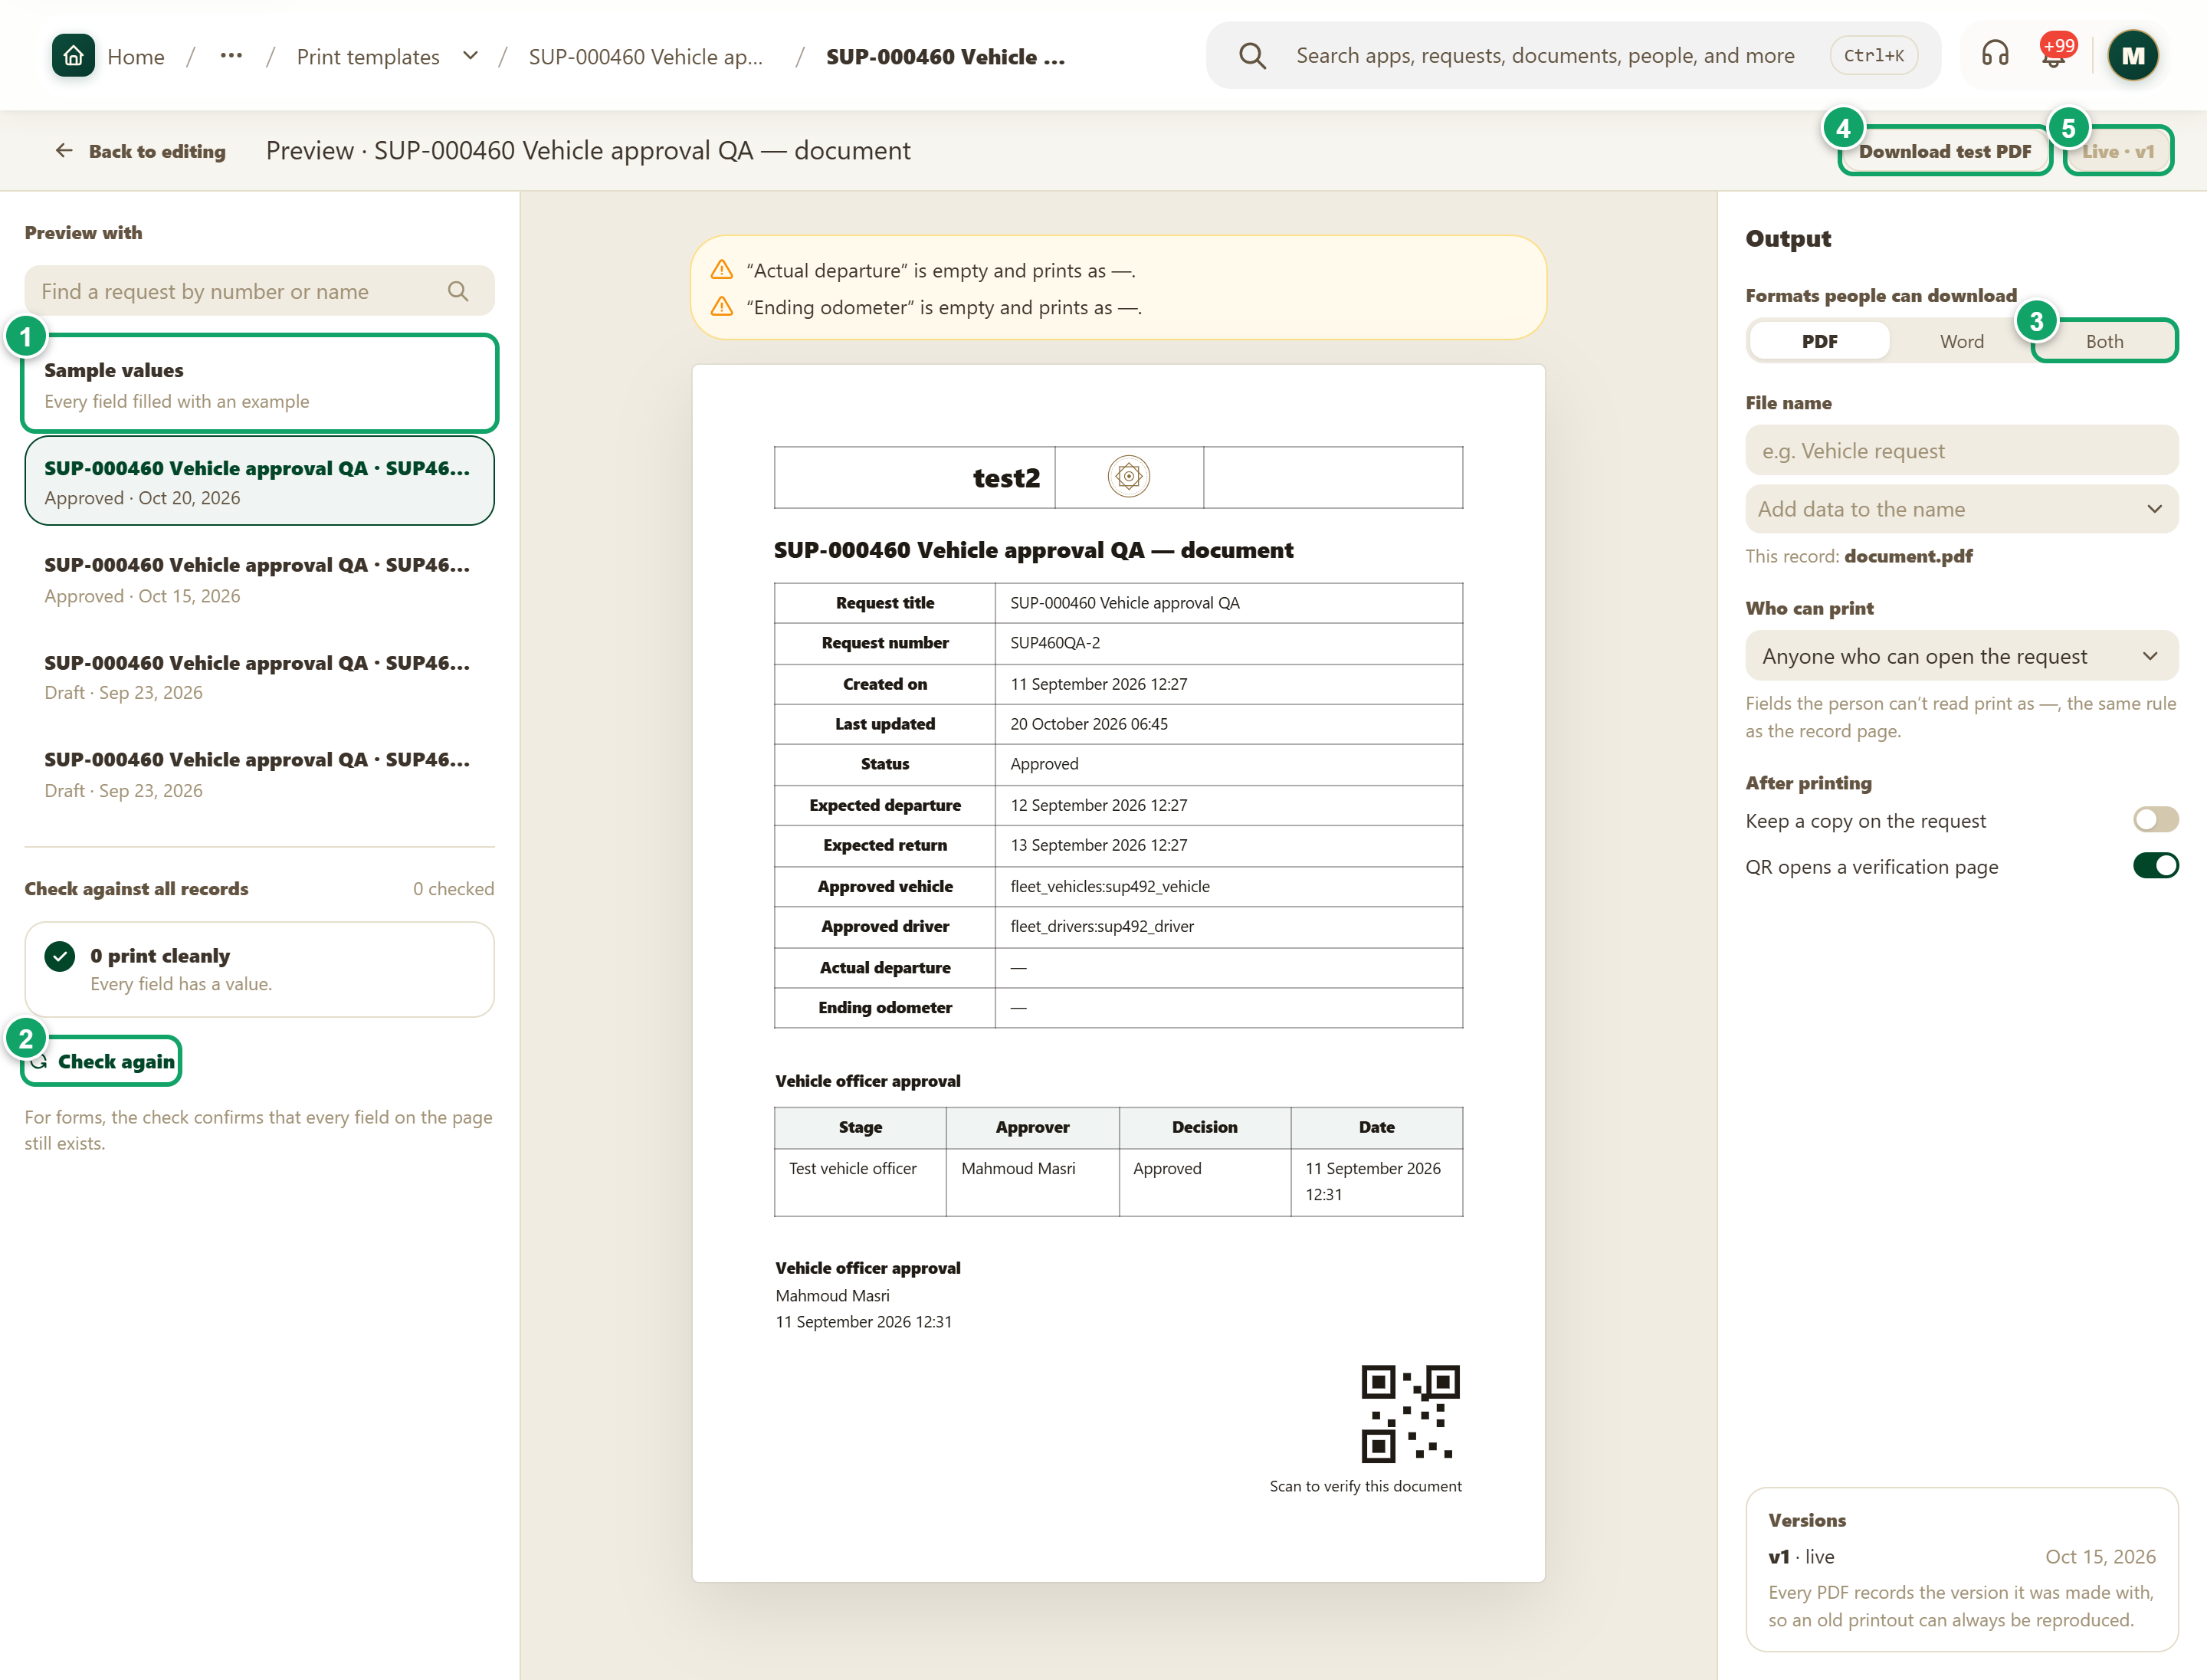
\includegraphics[width=0.95\linewidth,height=0.72\textheight,keepaspectratio]{figures/screens/ch06-print-publish-en.png}
\caption{The print template preview page}
\label{fig:builder-print-publish-screen}
\shotnote{The image shows the test template previewed on a real request on test2, with a notice above the document about two empty fields that will print as —. The page brings together preview, check and output, so you decide to publish while seeing the result. ① “Sample values”: the top of the list where you pick examples or a real record. ② “Check again”: reruns “Check against all records” after any change. ③ “Both”: allows downloading PDF and Word together. ④ “Download test PDF”: downloads the document for the chosen record. ⑤ The publish button: shows “Live · v1” because there are no unpublished changes.}
\end{figure}

\begin{table}[H]
\centering
\caption{The preview page}
\label{tab:builder-print-publish-preview}
\begin{tabularx}{\linewidth}{R{3.6cm} Y}
\rcHeaderRow
\thh{Part} & \thh{Content and action}\\
“Preview with” & Find a record by number or name, or choose “Sample values” to fill every field with an example.\\
“Check against all records” & Runs on its own when the page opens, and “Check again” reruns it after any change. It checks the newest records you can open and tells you how many print cleanly and which miss a field or hide it from some people. For forms it only confirms that every field still exists.\\
“Download test PDF” & Downloads the document for the chosen record; it does not work before a record is chosen.\\
“Output” & “Formats people can download”: PDF, Word or “Both”; the “File name” with “Add data to the name”; “Who can print”: anyone who opens the record or only those who edit it; “Keep a copy on the record”; and “QR opens a verification page”.\\
“Publish vN” & Publishes the template so new prints use this version. The “Versions” button in the builder header lists published versions and their dates.\\
\end{tabularx}
\end{table}

\begin{table}[H]
\centering
\caption{Printing from a record}
\label{tab:builder-print-publish-record}
\begin{tabularx}{\linewidth}{R{3.6cm} Y}
\rcHeaderRow
\thh{Action} & \thh{What happens}\\
“Print” → “Choose a document” & Lists the published templates, the default one first.\\
“Download PDF”, “Print now” or “Download Word” & Creates the document in the formats you allowed under “Output”.\\
“Printed copies” & Lists the saved copies if you turned on keeping a copy on the record.\\
“Fill these fields before printing” & Appears when a field set to “Stop print” is empty.\\
Bulk print & Select several records in the record type's table and press “Print”, then choose one PDF, one Word file or a zip file. Records you cannot open are skipped and listed.\\
\end{tabularx}
\end{table}

\begin{figure}[H]
\centering
\begin{tikzpicture}[node distance=0.5cm]
\node[stepBox] (a) {Preview with a record};
\node[stepBox,below=of a] (b) {Check against all records};
\node[stepBox,below=of b] (c) {Set the output};
\node[stepBox,below=of c] (d) {Publish the version};
\node[stepBox,below=of d] (e) {Print from the record};
\draw[flowsTo] (a) -- (b);
\draw[flowsTo] (b) -- (c);
\draw[flowsTo] (c) -- (d);
\draw[flowsTo] (d) -- (e);
\end{tikzpicture}
\rclegend
\caption{From preview to the first printed copy}
\label{fig:builder-print-publish-flow}
\shotnote{The diagram places the full check after previewing a single record, because one correct record does not guarantee that the others have the same fields. Setting the output comes before publishing, since it decides the formats, who prints and whether the document carries a verification code.}
\end{figure}

\subsection{Steps and check}
\begin{enumerate}
\item Press “Preview with a record” and find a real record in “Preview with”.
\item Read the result of “Check against all records”, press “Check again” after any change, and deal with any missing or deleted fields it reports.
\item Set the “Output”: formats, file name, “Who can print”, keeping a copy and the verification code.
\item Press “Download test PDF” and review the file, then press “Publish vN”.
\item Open a record, press “Print”, choose the template and download the document.
\end{enumerate}

\textbf{Check and recovery:} the message “Published vN. New prints use this version.” should appear, and the template should show in “Choose a document”. If “Your latest changes couldn’t be saved, so nothing was published” appears, fix the saving problem and publish again. If a field prints as —, it may be empty or the person may not be allowed to read it.

\clearpage
\section{Document verification page}
\label{sec:builder-feature-print-verify}

When you turn on “QR opens a verification page” in a template's output, every printed document carries its own verification code. Scanning the code opens a public page that needs no sign-in and shows the document as issued with its main details. That way anyone who receives the paper, inside or outside the organization, can confirm it was really issued and that its content has not changed. But the code confirms the document that was issued, not the paper it appears on, so the reader compares the two.

\textbf{Path and who uses it:} scanning the QR code printed on the document, or opening its link. Used by whoever receives the document; the template designer turns it on under “Output”.

\begin{rcnote}[Example: Horizon]
The Aleppo Branch receives the printed visit sheet for request HZN-VR-0001, and the reception employee scans its code. The “Code confirmed” page appears with the document as issued, and the employee compares the date and names with the paper in hand.
\end{rcnote}

\begin{figure}[H]
\centering
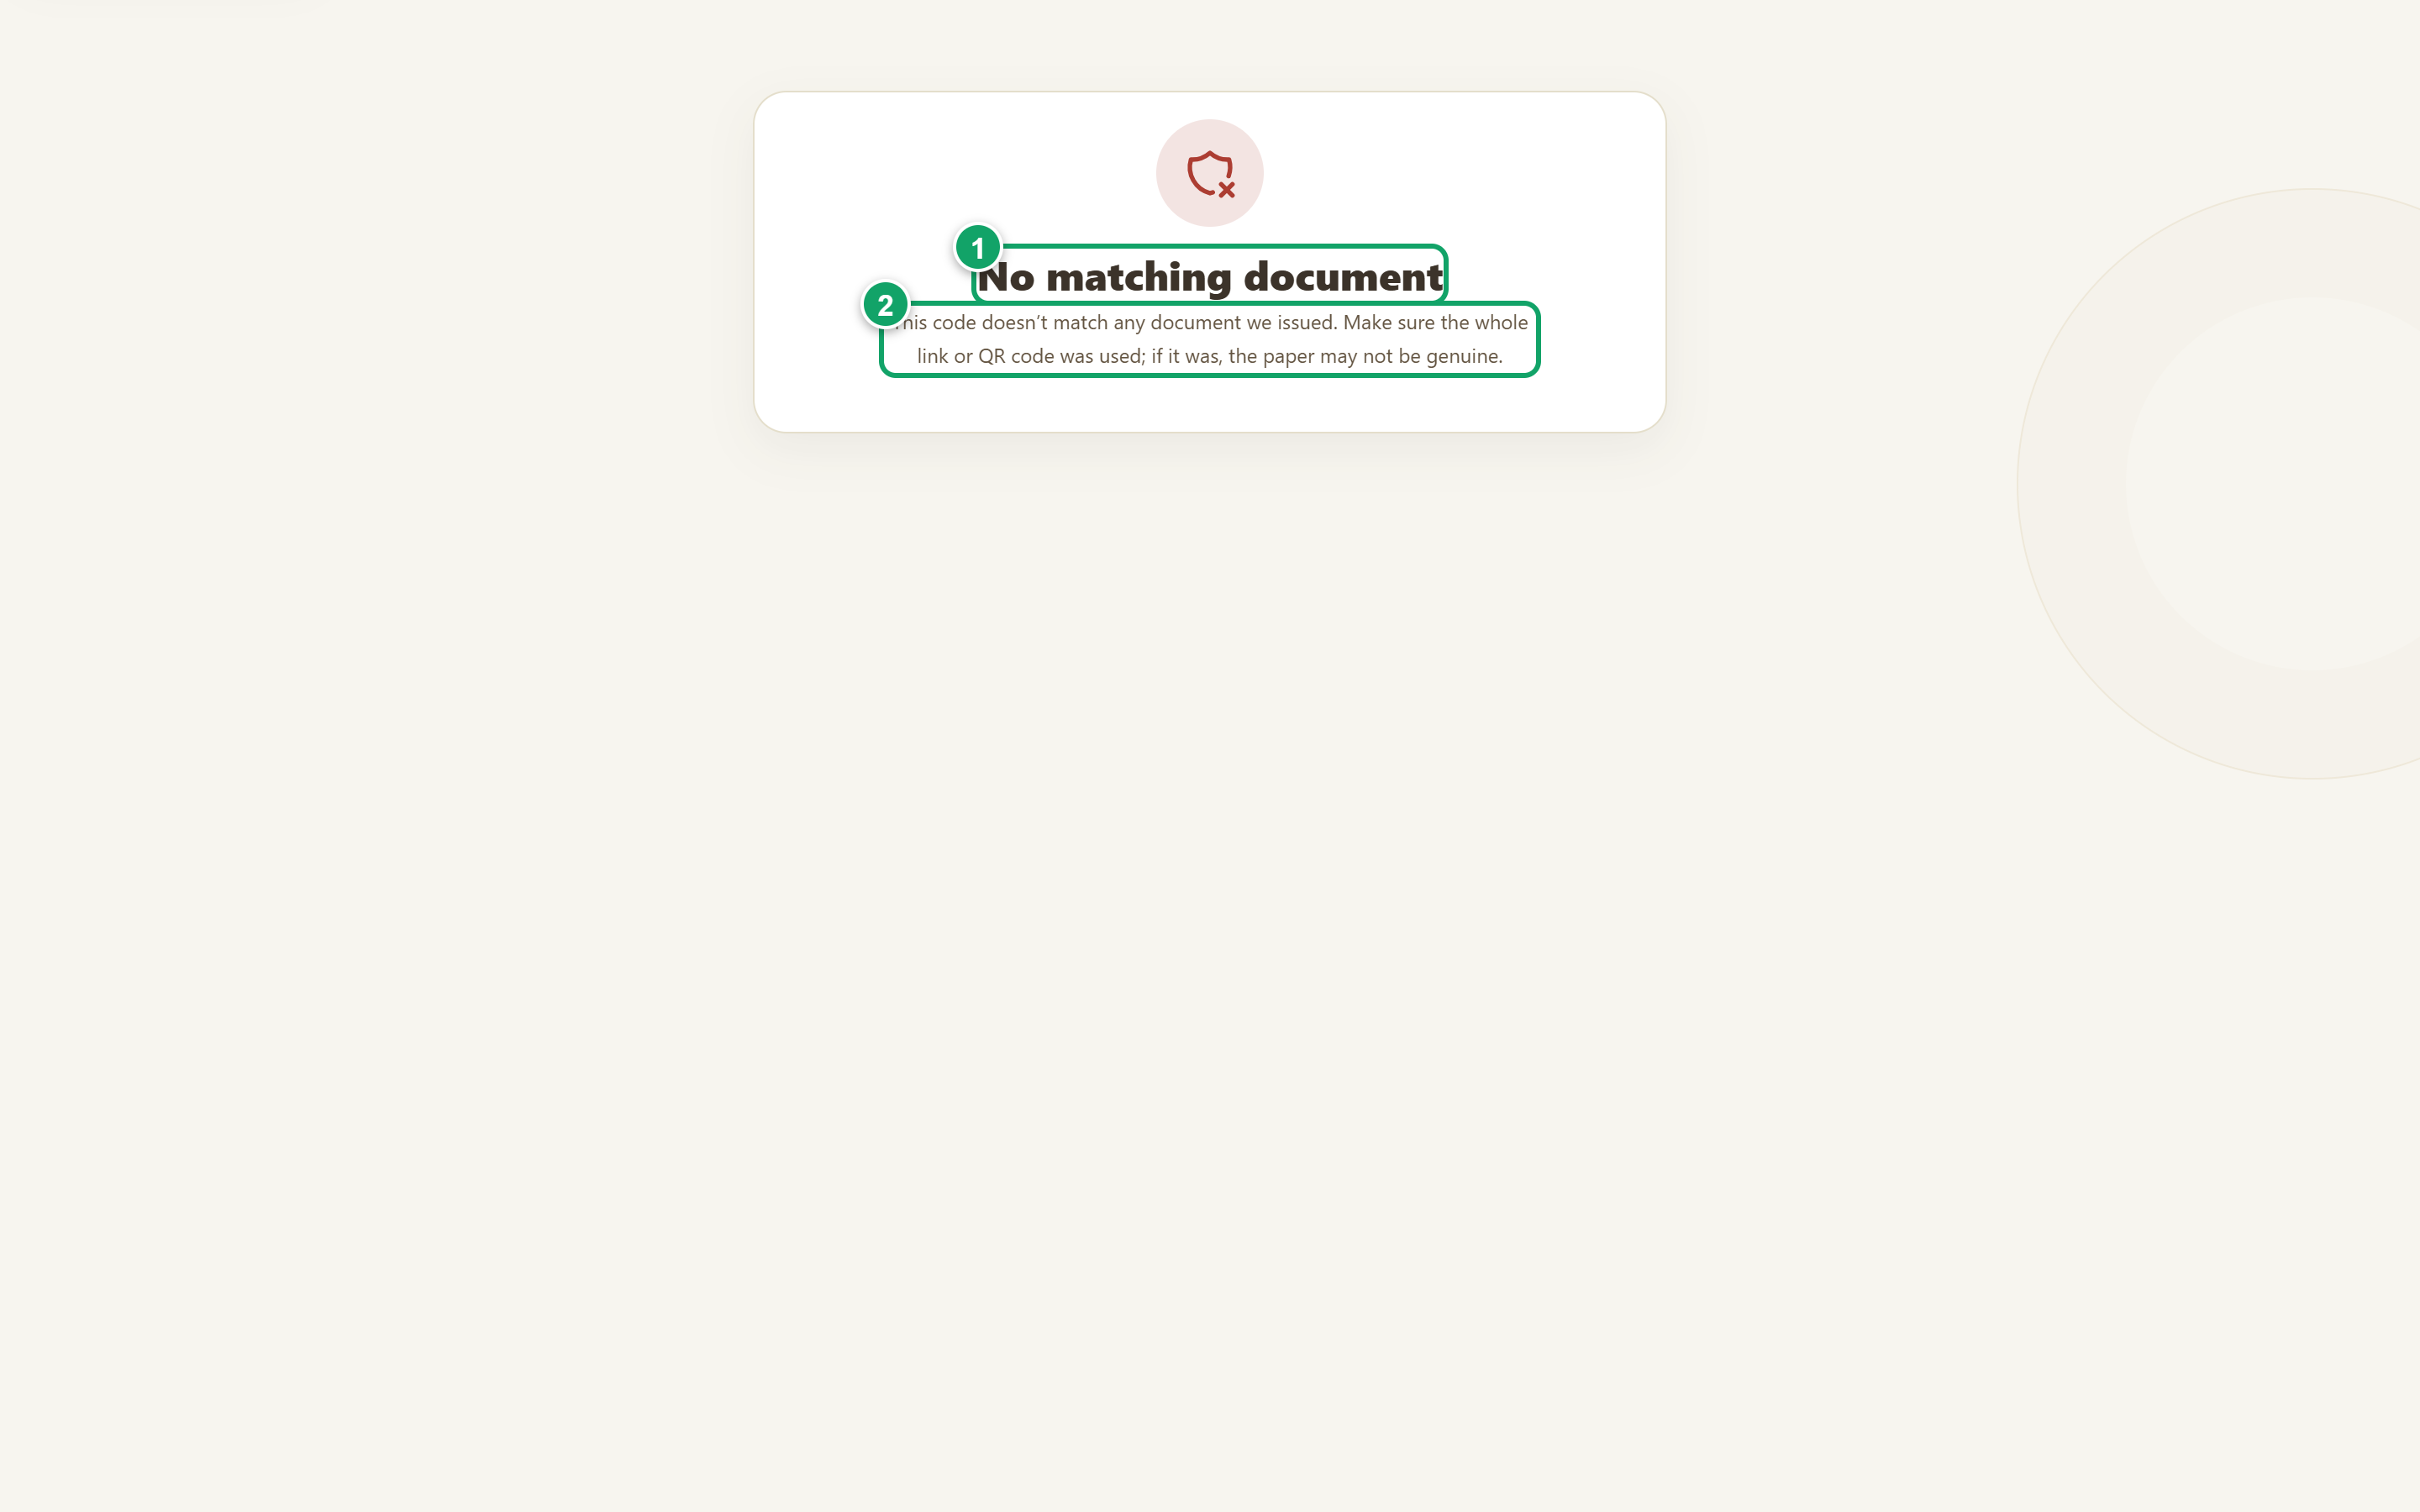
\includegraphics[width=0.95\linewidth,height=0.72\textheight,keepaspectratio]{figures/screens/ch06-print-verify-en.png}
\caption{The verification page with an invalid code}
\label{fig:builder-print-verify-screen}
\shotnote{The image shows the public verification page opened with a sample code that matches no document, since capturing it with a real code requires printing an actual document. It is the result someone sees with a forged paper or an incomplete link, and it shows without signing in. ① “No matching document”: the check result. ② The guidance text: asks you to make sure the whole link or code was used before judging the paper.}
\end{figure}

\begin{table}[H]
\centering
\caption{What the verification page shows}
\label{tab:builder-print-verify-results}
\begin{tabularx}{\linewidth}{R{3.6cm} Y}
\rcHeaderRow
\thh{Result} & \thh{What it means}\\
“Code confirmed” & The organization issued the code for this document. “Document details” show “Document”, “Issued by”, “Issued on”, “Template version” and “File fingerprint”.\\
“The document as issued” & The document's text as printed. Signatures show as placeholders naming the signer, and the QR code is left out.\\
“Check a file you received” & Choose a PDF or Word file you received, and the page tells you whether it is the exact file that was issued. The file stays on your device.\\
“No matching document” & The code matches no issued document; make sure the whole link or code was used, otherwise the paper may not be genuine.\\
“We couldn’t check this document right now” & A temporary problem that does not mean the document is not genuine; try again in a moment.\\
\end{tabularx}
\end{table}

\begin{rcwarn}[Compare the paper with the document shown]
If a name, number, date or amount differs between the paper and the document shown, the paper was changed after it was issued. If the document was printed with others in one file through bulk print, its file cannot be checked; compare the content only.
\end{rcwarn}

\begin{figure}[H]
\centering
\begin{tikzpicture}[node distance=0.5cm]
\node[stepBox] (a) {Turn on verification in Output};
\node[stepBox,below=of a] (b) {Print the document with a QR code};
\node[stepBox,below=of b] (c) {Scan the code};
\node[stepBox,below=of c] (d) {Compare the paper with the document as issued};
\draw[flowsTo] (a) -- (b);
\draw[flowsTo] (b) -- (c);
\draw[flowsTo] (c) -- (d);
\end{tikzpicture}
\rclegend
\caption{From printing to verification}
\label{fig:builder-print-verify-flow}
\shotnote{The diagram shows that verification starts with a decision by the template designer: a document carries no code unless it is turned on. The steps end with the comparison because the page proves what was issued, and the reader still has to confirm that the paper matches it.}
\end{figure}

\subsection{Steps and check}
\begin{enumerate}
\item Turn on “QR opens a verification page” in “Output”, and place a “QR code” block in the template or in the letterhead.
\item Publish the template and print a test document from a record.
\item Scan the code with your phone and make sure “Code confirmed” appears.
\item Compare “The document as issued” with the paper, and try “Check a file you received” with the PDF you downloaded.
\end{enumerate}

\textbf{Check and recovery:} the page should open without signing in, and its details should match the paper. If the code does not print on the document, verification is off for this template, so turn on “QR opens a verification page” under “Output”. If “This document is too large to verify by QR” appears when printing, turn off verification for the template or print fewer rows.

\clearpage
\section{Identities \& letterheads}
\label{sec:builder-feature-identities}

An identity is the organization's logo, name, colours and official details, such as its registration number and address. A letterhead is the page header and footer shown in printed documents. This page keeps both in one place, so print templates and official correspondence share them, and any change here shows in all of them at the next print.

\textbf{Path and who uses it:} “Builder” → “Core” → “Identities \& letterheads”. Used by those who manage how the organization's documents look.

\begin{rcnote}[Example: Horizon]
The system administrator uploads Horizon's logo and adds its official details to the default identity, then creates a letterhead whose header shows on the first page only, so the visit sheet prints with the company logo without redesigning it in every template. They upload the logo in ③ and save from ④, then create the letterhead from ②.
\end{rcnote}

\begin{figure}[H]
\centering
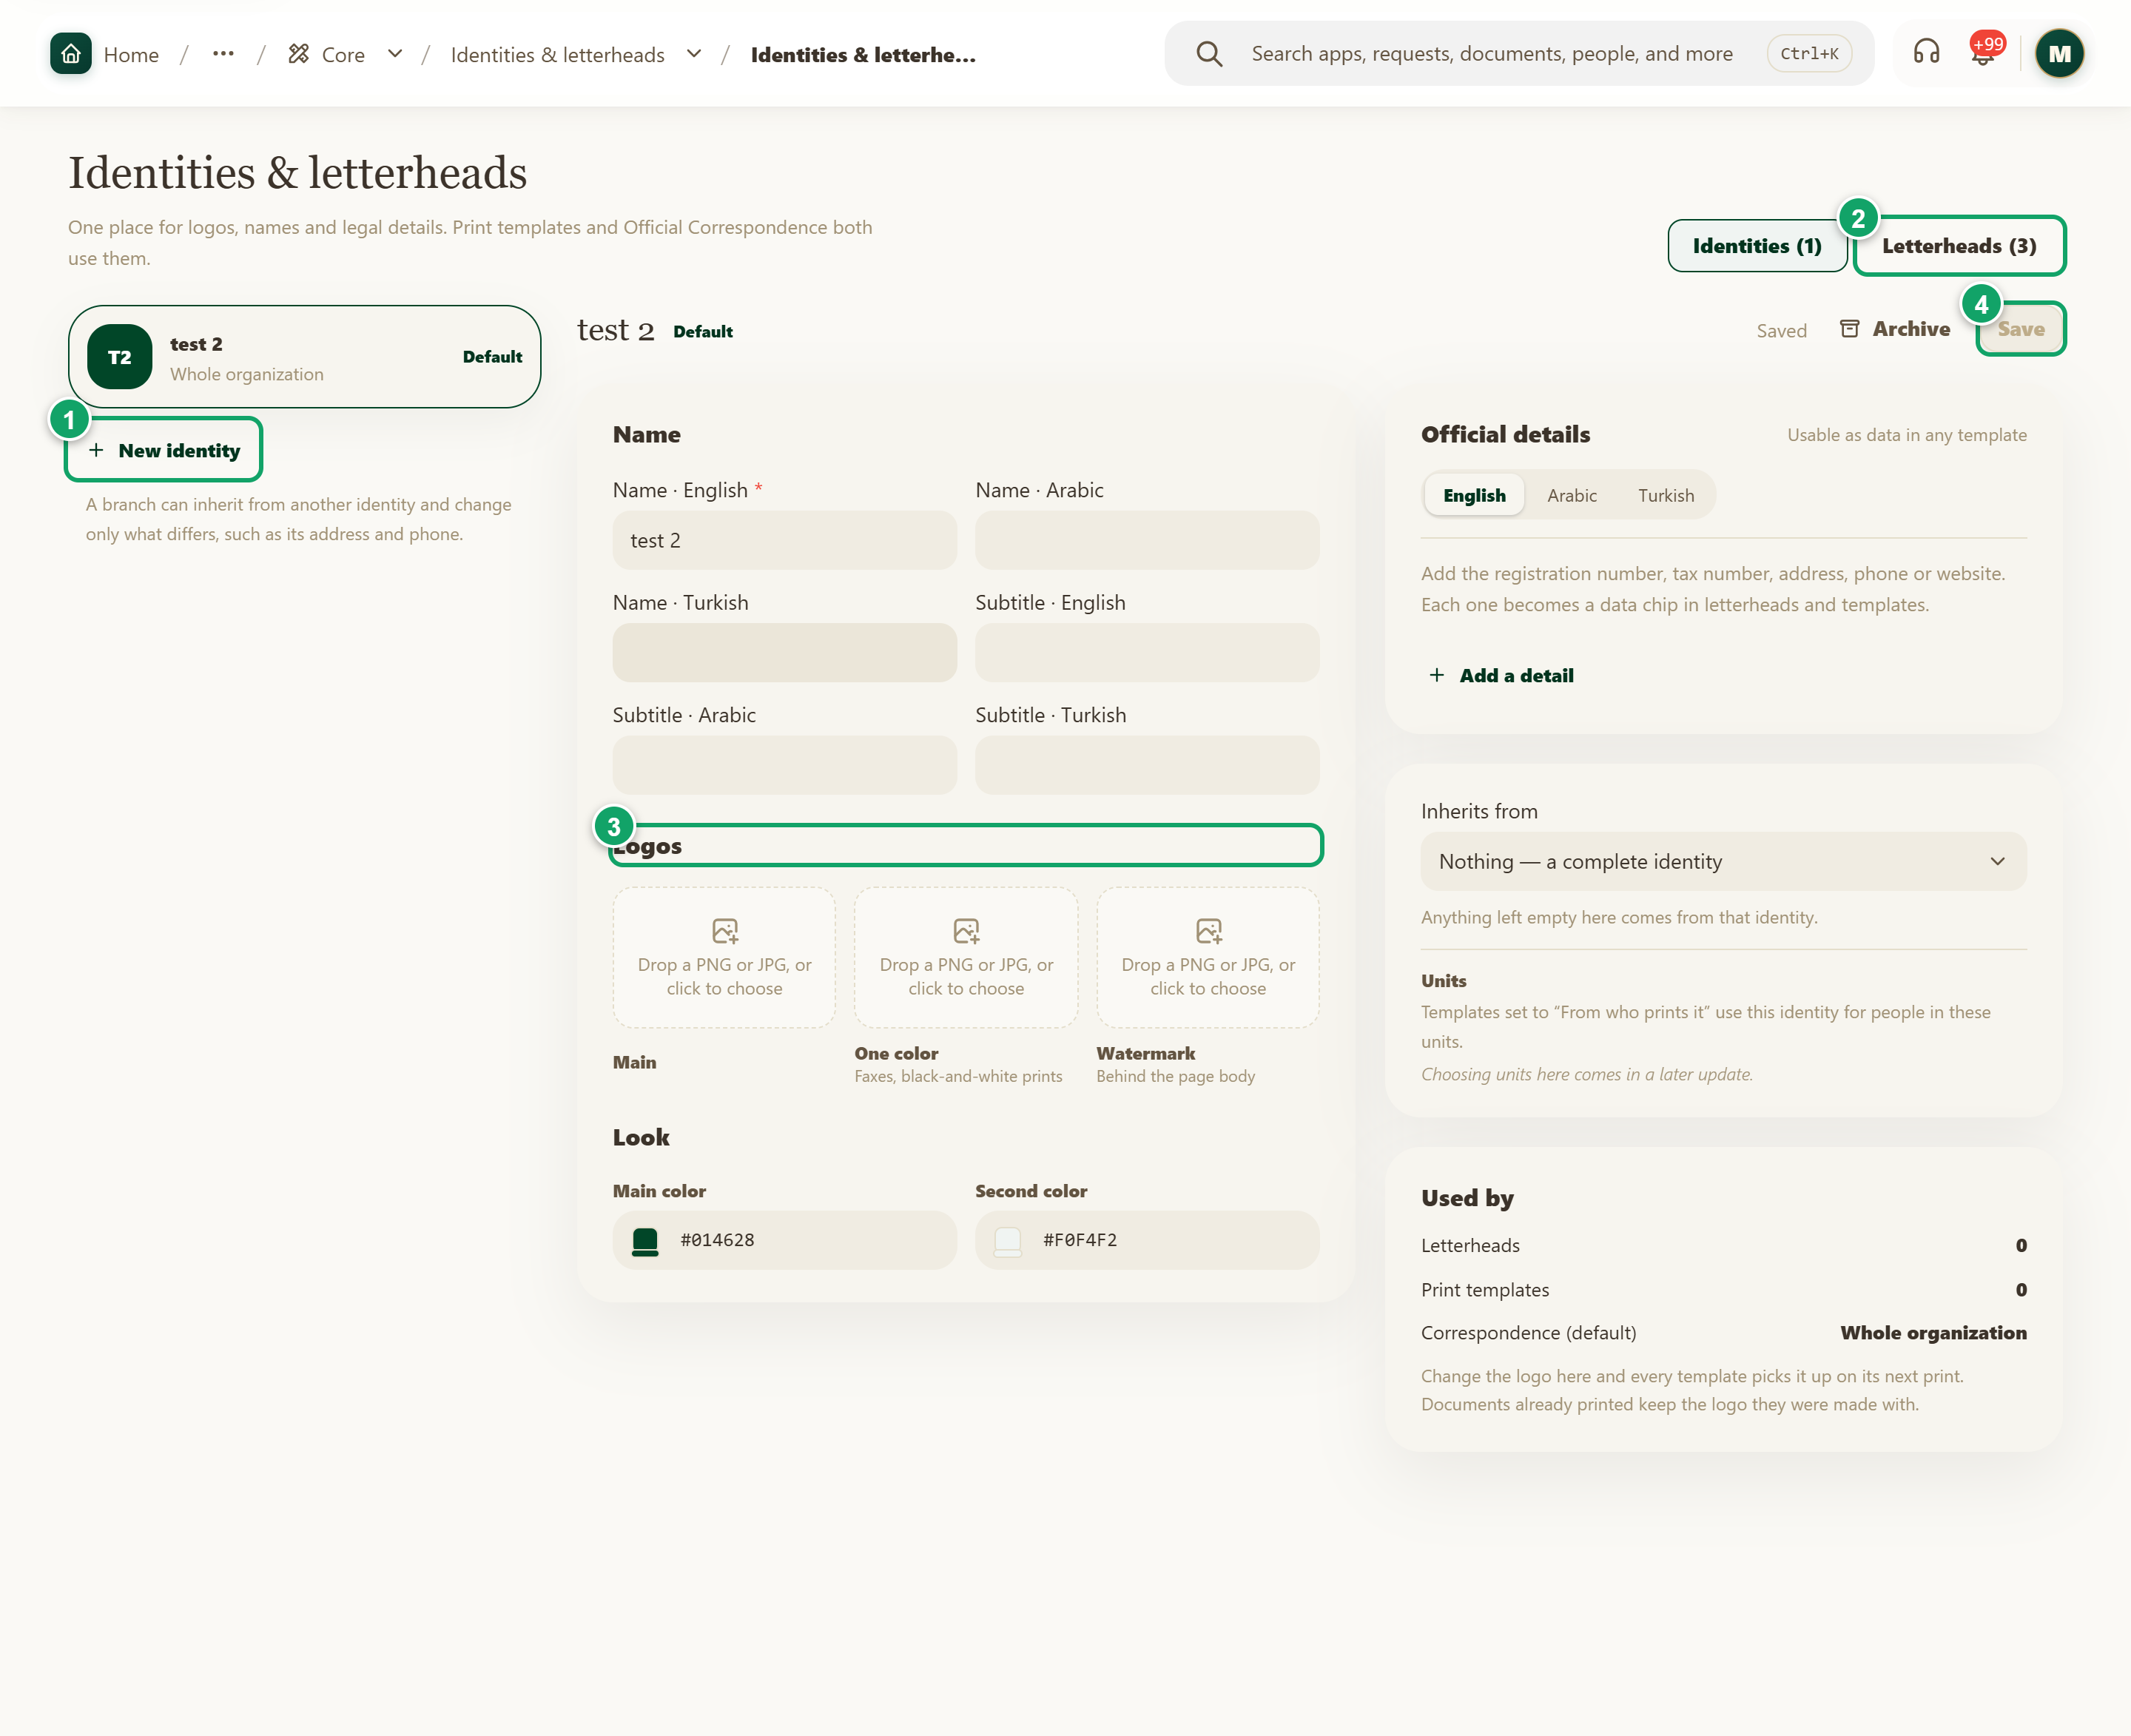
\includegraphics[width=0.95\linewidth,height=0.72\textheight,keepaspectratio]{figures/screens/ch06-identities-en.png}
\caption{The “Identities \& letterheads” page}
\label{fig:builder-identities-screen}
\shotnote{The page shows the organization’s default identity and its fields, here the test organization’s identity. ① “New identity”: creates another identity, such as a branch identity. ② “Letterheads”: the shared letterheads tab. ③ “Logos”: main, one-color and watermark logos. ④ “Save”.}
\end{figure}


\begin{table}[H]
\centering
\caption{What do you find here?}
\label{tab:builder-identities-data}
\begin{tabularx}{\linewidth}{R{3.6cm} Y}
\rcHeaderRow
\thh{Part} & \thh{Content and action}\\
Identities & Each identity has a “Name” and “Subtitle” in every language, “Logos” (main, one color, watermark), a “Look” with two colours, and “Official details”.\\
Inherits from & Lets an identity take what it does not set from another identity, such as a branch identity inheriting from the organization's.\\
Used by & Shows the letterheads, print templates and correspondence that rely on the identity.\\
Letterheads & The list of shared letterheads, each with the number of templates using it, offering “Edit”, “Duplicate”, “Make default” and “Archive”.\\
\end{tabularx}
\end{table}

\begin{figure}[H]
\centering
\begin{tikzpicture}[node distance=0.5cm]
\node[entity] (id) {Identity};
\node[entityOpt,below=0.7cm of id] (lh) {Letterhead};
\node[entityOpt,below right=0.7cm and 0.3cm of lh] (print) {Print templates};
\node[entityOpt,below left=0.7cm and 0.3cm of lh] (corr) {Official correspondence};
\draw[dependsOnOpt] (id) -- (lh);
\draw[dependsOnOpt] (lh.south) -- ++(0,-0.3) -| (print.north);
\draw[dependsOnOpt] (lh.south) -- ++(0,-0.3) -| (corr.north);
\end{tikzpicture}
\rclegend
\caption{From identity to the printed document}
\label{fig:builder-identities-model}
\shotnote{The figure shows that the identity feeds the letterhead, and the letterhead is shared by print templates and official correspondence. So change the logo or official details in the identity once, and the change shows in every document printed afterwards; review “Used by” before any change.}
\end{figure}

\subsection{Steps and check}
\begin{enumerate}
\item Open “Identities \& letterheads”, choose the default “Whole organization” identity or create a “New identity”.
\item Write the name in each language, upload the logos as PNG or JPG, add the official details, then press “Save”.
\item Open “Letterheads”, create a “New letterhead”, and choose its items and where they show.
\end{enumerate}

\textbf{Check and recovery:} print a test document from a template using the letterhead; the logo and new details should appear. If you cannot archive an identity, make another identity the default first, because the default identity cannot be archived.

\clearpage
\section{Letterhead editor}
\label{sec:builder-feature-letterheads}

A letterhead is a page header and footer you design once, then print templates and official correspondence use them. The letterhead editor shows a sheet with two zones: the “Header” at the top and the “Footer” at the bottom, with the place for each template's content between them. You add text you write yourself to both zones, or identity and document data that changes with every print, such as the organization's name, the print date and the page number. Any change you save here shows in every template that uses the letterhead and in official letters too.

\textbf{Path and who uses it:} “Builder” → “Core” → “Identities \& letterheads” → “Letterheads” → “New letterhead” or “Edit”. Used by those who manage how the organization's documents look.

\begin{rcnote}[Example: Horizon]
The system administrator creates a letterhead named “Horizon letterhead”, places the logo and name in its header, and the Head Office Damascus address and the page number in its footer. They set the header to show on the first page only and the footer on every page, then press “Save”. They write the name in ①, insert the logo from ② and the page number from ③, set the pages beside ④, then save with ⑤.
\end{rcnote}

\begin{figure}[H]
\centering
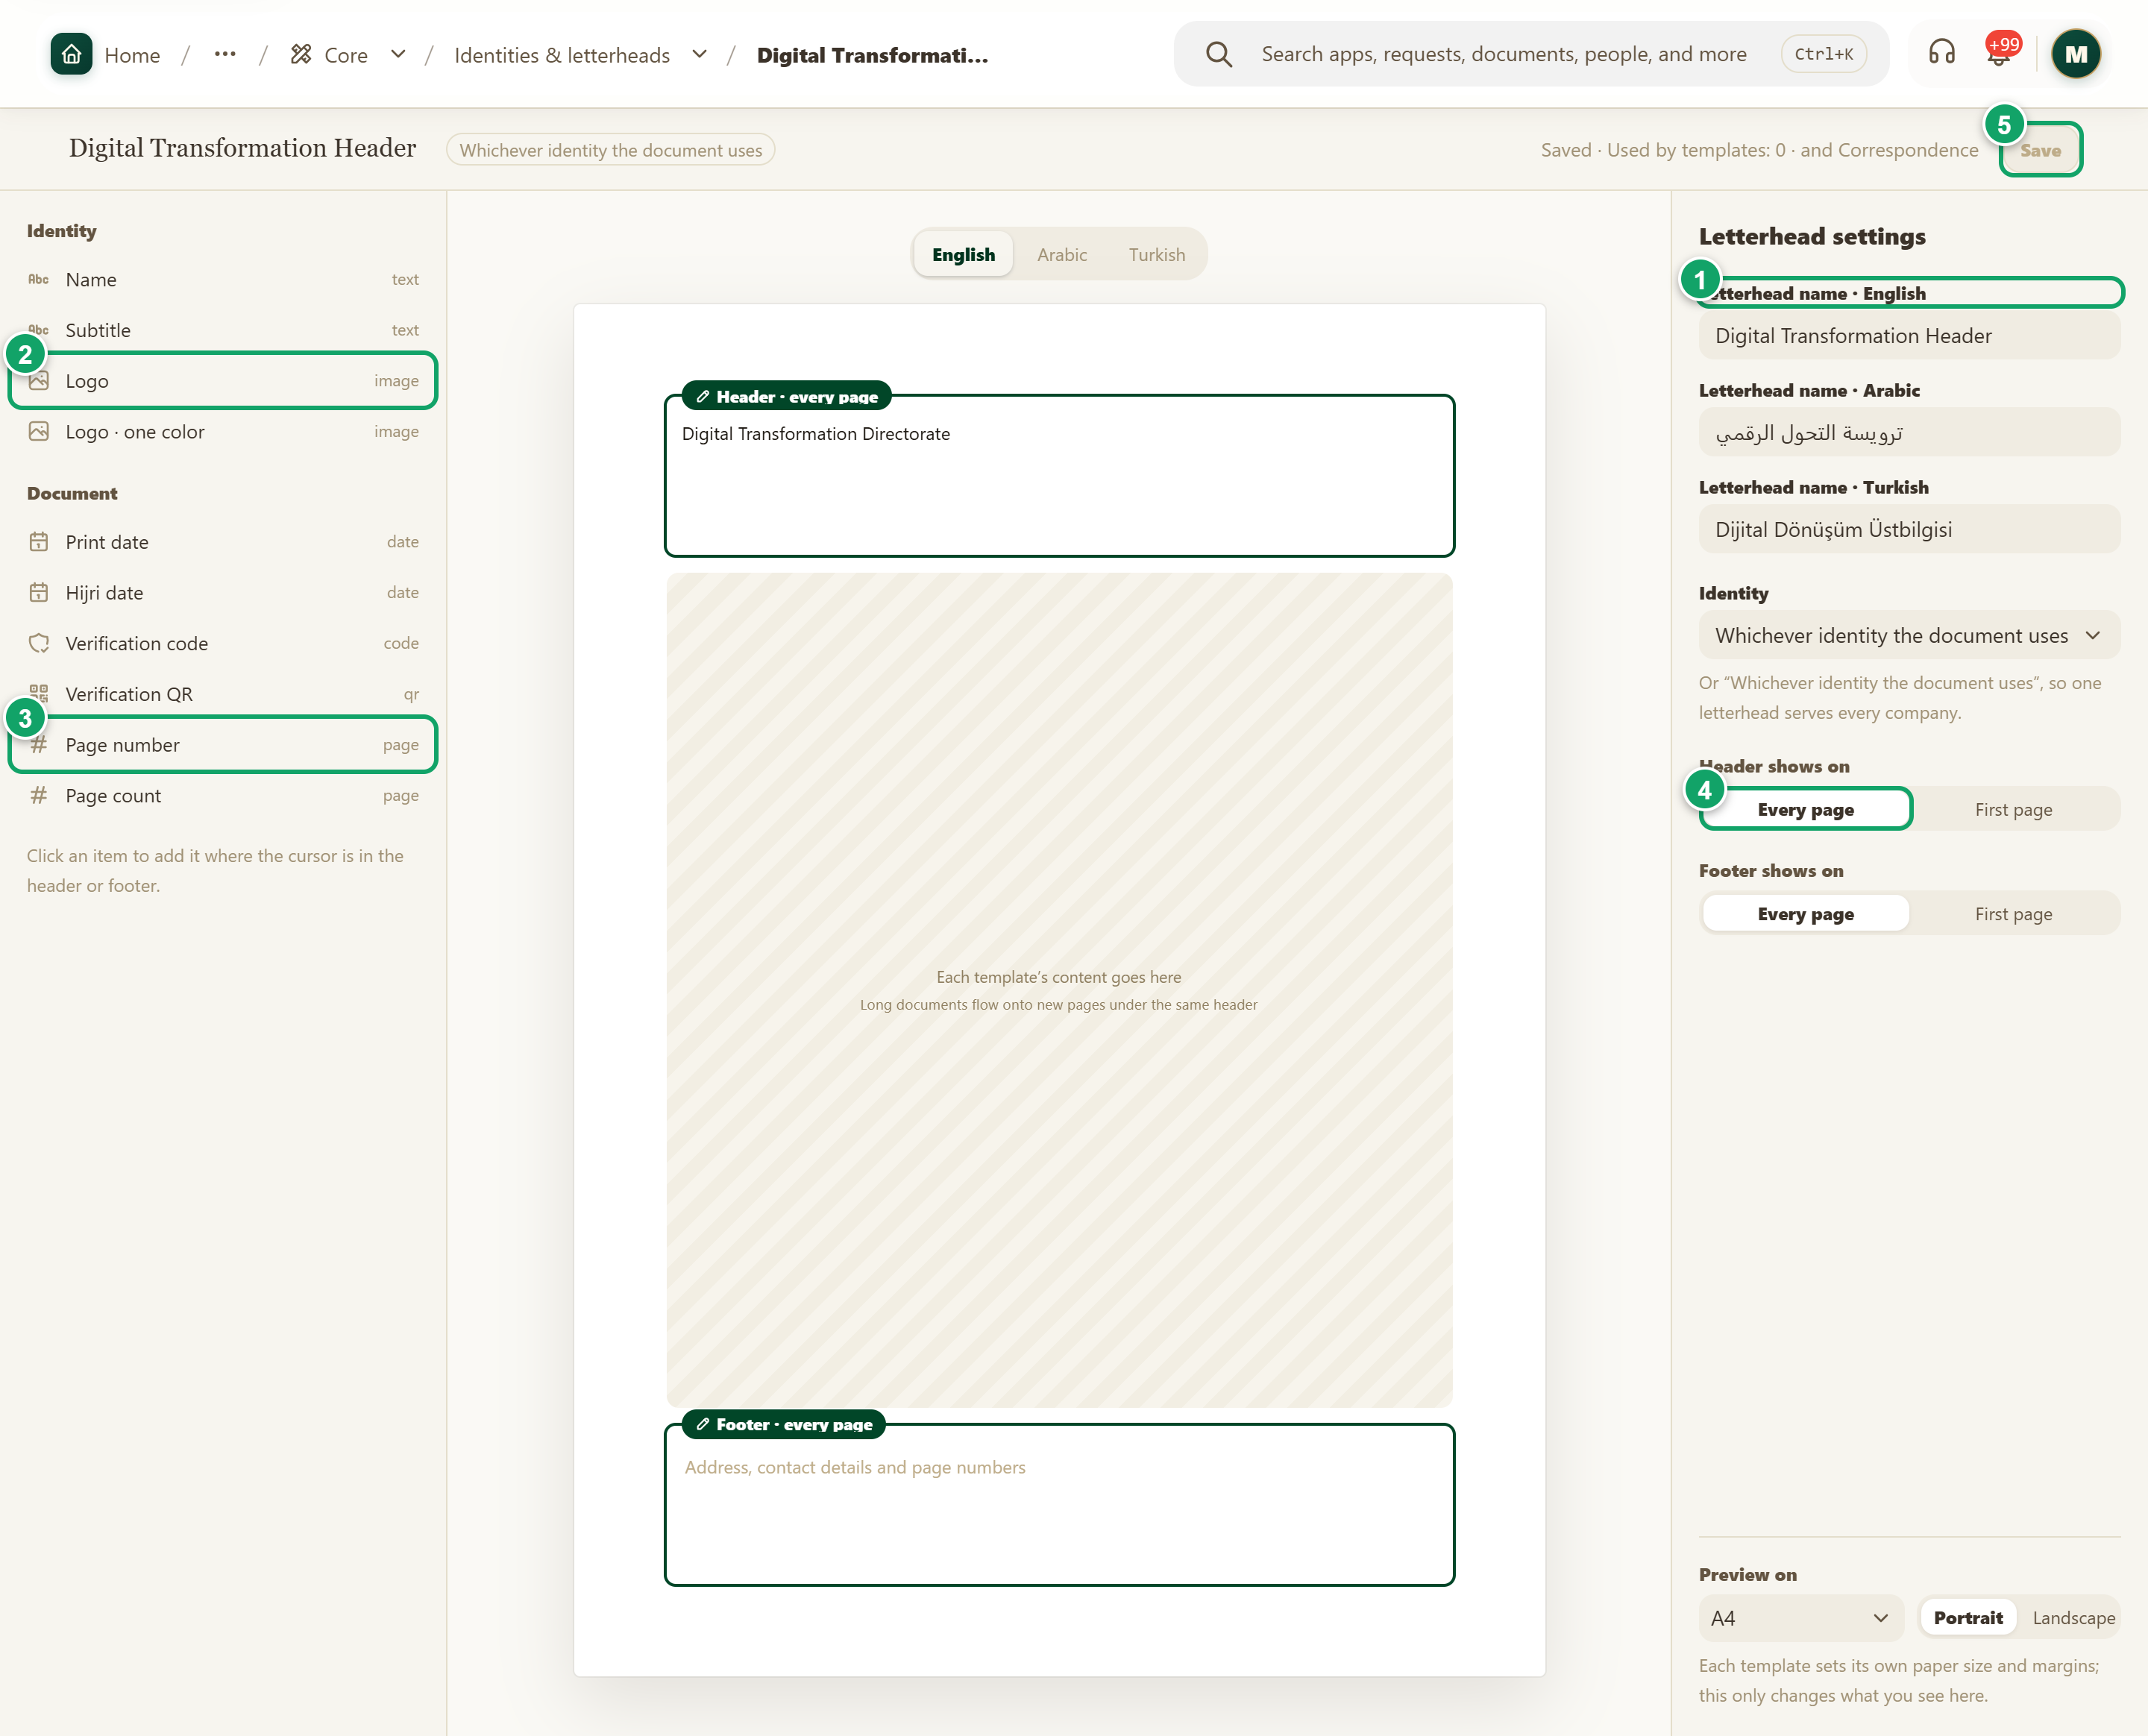
\includegraphics[width=0.95\linewidth,height=0.72\textheight,keepaspectratio]{figures/screens/ch06-letterheads-en.png}
\caption{The letterhead editor for an existing letterhead}
\label{fig:builder-letterheads-screen}
\shotnote{The image shows a test letterhead on test2 open in the editor on English, with a line of text in its header and an empty footer. The line beside the save button shows how many templates use the letterhead, so you know the effect of a change before saving. ① “Letterhead name · English”: the name shown when choosing the letterhead in templates. ② “Logo”: inserted from identity data at the cursor. ③ “Page number”: from document data. ④ “Every page”: the pages the header shows on. ⑤ “Save”: saves the letterhead for everyone using it.}
\end{figure}

\begin{table}[H]
\centering
\caption{The “Data” list in the editor}
\label{tab:builder-letterheads-data}
\begin{tabularx}{\linewidth}{R{3.6cm} Y}
\rcHeaderRow
\thh{Group} & \thh{Items}\\
“Identity” & “Name”, “Subtitle”, “Logo” and “Logo · one color”, plus every detail added under the identity's “Official details”, such as the tax number.\\
“Document” & “Print date”, “Hijri date”, “Verification code”, “Verification QR”, “Page number” and “Page count”.\\
\end{tabularx}
\end{table}

You add an item by pressing it, and it is inserted where the cursor is in the header or footer.

\begin{table}[H]
\centering
\caption{“Letterhead settings”}
\label{tab:builder-letterheads-settings}
\begin{tabularx}{\linewidth}{R{3.6cm} Y}
\rcHeaderRow
\thh{Setting} & \thh{What it sets}\\
“Letterhead name” & A name shown when choosing the letterhead in templates, written in each of the organization's languages.\\
“Identity” & A specific identity, or “Whichever identity the document uses” so one letterhead serves every identity.\\
“Header shows on” and “Footer shows on” & “Every page” or “First page”.\\
“Preview on” & “Portrait” or “Landscape”; it changes only what you see in the editor, because each template sets its own paper and margins.\\
“Letterhead language” & Tabs shown when the organization has more than one language, so you design the letterhead for each language.\\
\end{tabularx}
\end{table}

\begin{figure}[H]
\centering
\begin{tikzpicture}[node distance=0.5cm]
\node[stepBox] (a) {New letterhead};
\node[stepBox,below=of a] (b) {Write the header and footer};
\node[stepBox,below=of b] (c) {Insert identity and document data};
\node[stepBox,below=of c] (d) {Set the identity and pages};
\node[stepBox,below=of d] (e) {Save and choose it in templates};
\draw[flowsTo] (a) -- (b);
\draw[flowsTo] (b) -- (c);
\draw[flowsTo] (c) -- (d);
\draw[flowsTo] (d) -- (e);
\end{tikzpicture}
\rclegend
\caption{Setting up a shared letterhead}
\label{fig:builder-letterheads-flow}
\shotnote{The diagram shows that a letterhead is designed once and then chosen in each template, so it is never rewritten for every document. Identity data is inserted rather than typed as fixed text, because a change to the logo or address in the identity then reaches the letterhead automatically.}
\end{figure}

\subsection{Steps and check}
\begin{enumerate}
\item Open “Identities \& letterheads”, then “Letterheads”, and press “New letterhead”.
\item Write the “Letterhead name” and choose the “Identity” in “Letterhead settings”.
\item Click inside the header, write what you want, then add the “Logo” and “Name” from the “Data” list.
\item Click inside the footer and add the address or contact details and the “Page number”.
\item Choose the pages the header and footer show on, then press “Save”.
\end{enumerate}

\textbf{Check and recovery:} the status should change to “Saved” with the number of templates using the letterhead, and the letterhead should appear in the list. If “Give the letterhead a name.” appears, write the name then save. If “Print templates still use this letterhead” appears when archiving, choose another letterhead in those templates first.
